%------book书籍类,openany选项表示可从任何页开始新章节------
\documentclass[a4paper,12pt,twoside,openany]{book}
%---------导言文章格式设置-------
%-----宏包-----------
\usepackage{titletoc,titlesec,fancyhdr} %--版式--
\usepackage[left=1in,right=1in,top=1.25in,bottom=1in,headheight=16pt]{geometry} %-页面设置
\usepackage[colorlinks,linkcolor=black,anchorcolor=black,citecolor=black]{hyperref}%-超链接
\usepackage{xeCJK,fontspec} %--字体---
\usepackage[font=small,labelsep=quad]{caption}
\usepackage[font=small]{subcaption} %引用
\usepackage[super,square,numbers,sort&compress]{natbib}%--引用上标设置-
\usepackage{amsmath,amssymb,amsthm,esint,mathrsfs,amsfonts,cases,bm,array} %--数学环境----
\usepackage{booktabs,multirow,diagbox} %---三线表格--
\usepackage{graphicx,float,enumerate,multicol,color}%--图片等--
\usepackage{indentfirst,xpatch,setspace}%--行距缩进等
%-----------------------------------------------------
%-----------中英文字体设置----------------
\setmainfont{Times New Roman}
\setsansfont{Arial}
\setmonofont{Courier New}
\setCJKmainfont[BoldFont=方正小标宋_GBK,ItalicFont=方正楷体_GBK]{方正书宋_GBK}
\setCJKsansfont[BoldFont=方正大黑_GBK]{方正黑体_GBK}
\setCJKmonofont{方正仿宋_GBK}
\newCJKfontfamily\cukai{华文楷体}
\newCJKfontfamily \beiweikai{方正北魏楷书简体}
%\setCJKmainfont[ItalicFont={KaiTi}, BoldFont={SimHei}]{SimSun}
%\setCJKsansfont{KaiTi}
%\setCJKmonofont{FangSong}
%\setCJKmainfont[BoldFont={Adobe Heiti Std},
%    ItalicFont={Adobe Kaiti Std}]{Adobe Song Std}%
%\setCJKsansfont{Adobe Heiti Std}
%\setCJKmonofont{Adobe Fangsong Std}
%---------中英文设置结束-----------------
%----------------------格式定制-----------
%----------目录章节大标题拉近距离产生引导线--------------
\titlecontents{chapter}[1em]{\bfseries}{\contentslabel{1.5em}}
{\hspace*{-1.5em}}{\hspace{0.5em}\titlerule*[10pt]{.}\contentspage}
%--------正文之外的标题居中------
\titleformat{\chapter}{\centering\LARGE\bfseries}{\arabic{chapter}}{1em}{}
%---------修改章节定义,使章节页页眉格式改为fancy-----------
\xpatchcmd{\chapter}{\thispagestyle{plain}}{\thispagestyle{fancy}}{}{}
%-------章节标记定制为数字+名称---设置页眉页脚---------------
\pagestyle{fancy}
\renewcommand{\chaptermark}[1]{\markboth{\arabic{chapter}\quad #1}{}}
\fancyhf{}
\fancyhead[LO,RE]{\small~硕士学位论文~}
\fancyhead[RO]{\small~高速飞行器头罩湍流流场的气动光学效应分析~}
\fancyhead[LE]{\small~\leftmark~} %leftmark为一级标记,rightmark为二级标记
\fancyfoot[LE,RO]{\small~\thepage~}
%--------格式定制结束--------------
%----------------------间距设置------------
%-------章节标题与上下文距离、行间距-----------------
\titlespacing*{\chapter}{0.5em}{0pt}{15pt}
\titlespacing*{\section}{0.5em}{10pt}{10pt}
\titlespacing*{\subsection}{0.5em}{6pt}{6pt}
%\onehalfspacing%---1.5倍行间距---
\setlength{\parindent}{2em}%----首行缩进距离---

%---------间距设置结束-------------
%------------------其他设置------
\bibliographystyle{unsrtnat}%--参考文献格式,按引用顺序排序---
%-----------页脚----------
\usepackage[norule]{footmisc}
\usepackage{scrextend}
\deffootnote{1.5em}{1em}{\makebox[1.8em][l]{注\hspace{-0.3pt}\thefootnotemark:~~}}
\deffootnotemark{\textsuperscript{注\hspace{-0.1pt}\thefootnotemark}}
%\renewcommand{\thefootnote}{注\hspace{-0.2pt}\arabic{footnote}}%-脚注----
\graphicspath{{figure/}} %--设置图片路径---
%-------------目录等名称改为中文--------------------------
\renewcommand{\contentsname}{目~~录}
\renewcommand{\bibname}{参考文献}
\renewcommand{\indexname}{索引}
\renewcommand{\figurename}{图}
\renewcommand{\tablename}{表}
\renewcommand{\appendixname}{附录}
\renewcommand{\proofname}{证明}
\renewcommand{\listfigurename}{图~目~录}
\renewcommand{\listtablename}{表~目~录}
%-------去除citenum在方括号中间的空白-----------
\makeatletter
\DeclareRobustCommand\citenum
   {\begingroup
     \NAT@swatrue\let\NAT@ctype\z@\NAT@parfalse\let\textsuperscript\relax
     \NAT@citexnum[][]}
\makeatother 
%--------------格式设置完毕--------------------%--加载设置文档格式----
%\includeonly{} %--某些章节单独编译-----
%-----------------开始整篇文档---------------------    
\begin{document}
\setlength{\baselineskip}{20pt} %---1.5倍行间距---
%-------------封面、摘要、目录-----开始------
%-------封面开始-----------
%-----封面字体改变较多,记得要每页用{}括起来,否则影响正文--------
%----由于打印需要,封面每页后可以添加空白页保证单面打印--------
%----如果需要添加空白页,就把每页newpage后面去掉注释-----
%-----------------封面一--------------
\begin{titlepage}
%--------------抬头----------------------
%{
%\fontsize{10.95pt}{\baselineskip}\selectfont
% \makebox[3em]{分类号}\underline{\makebox[10em]{}}\hfill 密级\underline{\makebox[10em]{}}
%\par
%\makebox[3em]{UDC}\underline{\makebox[10em][l]{\footnotemark[1]}}\footnotetext[1]{注明《国际十进分类法UDC》的类号。}
%}
\vspace{5em}
\begin{center}
%--------------图标-----------------	

\includegraphics[width=0.95\textwidth]{body/titlepage/title.jpg}\\\vspace{1.2em}
%------------论文名和作者---------------------
{
\textbf{\cukai \fontsize{40pt}{\baselineskip}\selectfont 成教毕业设计报告}
}
%\par\vspace{3.3em}
%\noindent\underline{\makebox[\textwidth]{
%\sffamily\bfseries\fontsize{24pt}{\baselineskip}\selectfont 高速飞行器头罩湍流流场}}
%\vspace{1.5em}\par
%\noindent\underline{\makebox[\textwidth]{
%\sffamily\bfseries\fontsize{24pt}{
%\baselineskip}\selectfont 的气动光学效应分析}}\\
%{
%\vspace{0em}\normalsize\normalfont (题名和副题名)
%}\vspace{2em}\par
%\hspace{2em}\underline{\makebox[0.5\textwidth]{
%\cukai\fontsize{18pt}{\baselineskip}\selectfont \hspace{-1em}朱正天}}\\
%{\vspace{0em}\normalsize\normalfont (作者姓名)}
\end{center}
%---------------封面底部----------------------
%---------------总字体--------------
\par\vspace{10em}\fontsize{18pt}{\baselineskip}\selectfont 
%--------------格式---------------------
%\fbox{$\surd$}
\hspace{2.5em}
\makebox[0.2\textwidth][s]{\bfseries 类~~~~型}\hspace{.5em}\makebox[0.6\textwidth]{$\square$~~{设计说明书} \makebox[0pt][l]{$\checkmark$}$\square$毕业设计报告}
\par\vspace{.6em}
\hspace{2.5em}
\makebox[0.2\textwidth][s]{\bfseries 题~~~~目}\hspace{.5em}\underline{\makebox[0.6\textwidth]{国际电子贸易相关研究}}
\par\vspace{.6em}
\hspace{2.5em}
\makebox[0.2\textwidth][s]{\bfseries 学生姓名}\hspace{.5em}\underline{\makebox[0.6\textwidth]{姚枝叶}}
\par\vspace{.6em}
\hspace{2.5em}
\makebox[0.2\textwidth][s]{\bfseries 指导教师}\hspace{.5em}\underline{\makebox[0.6\textwidth]{
\cukai 赵~琦~~~~~~~}}
\par\vspace{.6em}
\hspace{2.5em}
\makebox[0.2\textwidth][s]{\bfseries 专~~~~业}\hspace{.5em}\underline{\makebox[0.6\textwidth]{
\cukai 工~学~硕~士}}
\par\vspace{.6em}
\hspace{2.5em}
\makebox[0.2\textwidth][s]{\bfseries 时~~~~间}\hspace{.5em}\underline{\makebox[0.6\textwidth]{
\cukai 2018年05月}}
\par\vspace{.6em}
\end{titlepage}
%----------插入空白页面-------
\newpage %\thispagestyle{empty} \mbox{}\newpage %
%%%%%%%%%%一下不需要
%%------------封面二--------------------
%{
%\thispagestyle{empty}
%\begin{minipage}{\textwidth}
%\quad\\\quad\\
%\end{minipage}
%%------------中文开头----------
%\begin{center}
%{\fontsize{20pt}{\baselineskip}\selectfont \CJKfontspec{华文新魏} 硕~~士~~学~~位~~论~~文}\\\vspace{6em}	
%{\fontsize{21pt}{\baselineskip}\selectfont\bfseries 
%高速飞行器头罩湍流流场的\\\vspace{.8em}气动光学效应分析}\\\vspace{8em}
%\end{center}
%%----------作者及其他--------------
%{\fontsize{18pt}{\baselineskip}\selectfont\bf
%\hspace{.25\textwidth}\makebox[0.22\textwidth][s]{作~~~~~者:}~~朱~正~天
%\par\vspace{1em}\noindent
%\hspace{.25\textwidth}\makebox[0.22\textwidth][s]{指导教师:}~~~赵~~琦~~~~~~教~授
%}\par\vfill
%\begin{center}
%\fontsize{18pt}{\baselineskip}\selectfont\bf 南~京~理~工~大~学\\
%	2016~年1~月\\
%\end{center} 
%\vspace{4em}
%}
%%----------插入空白页面-------
%\newpage %\thispagestyle{empty}\mbox{}\newpage %
%%----------------封面三--同封面二-------------------	
%{
%\thispagestyle{empty}
%\begin{minipage}{\textwidth}
%		\quad\\\quad\\
%\end{minipage}
%\begin{center}
%\fontsize{18pt}{\baselineskip}\selectfont
%{ Master Dissertation}\\\vspace{3.5em}
%{\fontsize{21pt}{\baselineskip}\selectfont\bfseries 
%Analysis of aero-optical effect around the\\\vspace{1.1em}
%turbulent flow field of the high-speed aircraft}
%\vspace{3em}\par
%\emph{By}\par \vspace{1.2em}\emph{\bf ZhengTian Zhu} \par \vspace{1.5em}
%\emph{Supervised by Prof}.\emph{\bf~~Qi Zhao}
%\par \vfill
%Nanjing University of Scirnce \& Technology\\
%January~,~2016\\
%\end{center}
%\vspace{4em}
%}
%%----------插入空白页面-------
%\newpage %\thispagestyle{empty}\mbox{}\newpage %
%%--------------封面四---------------
%{
%\thispagestyle{empty}
%\begin{minipage}{\textwidth}
%	\quad\\\quad
%\end{minipage}
%
%\begin{center}
%	\fontsize{19pt}{\baselineskip}\selectfont\bf 声~~明
%\end{center}
%{
%\fontsize{14.4pt}{1.5\baselineskip}\selectfont
%
%本学位论文是我在导师的指导下取得的研究成果,尽我所知,在本学位论文中,除了加以标注和致谢的部分外,不包含其他人已经发表或公布过的研究成果,也不包含我为获得任何教育机构的学位或学历而使用过的材料。与我一同工作的同事对本学位论文做出的贡献均已在论文中作了明确的说明。\vspace{2em}\par
%\noindent 研究生签名:\underline{\makebox[6em]{}}\hspace{7em}年~~~~~~~~月~~~~~~~~日
%}
%\par\vspace{5em}
%\begin{center}
%	\fontsize{19pt}{\baselineskip}\selectfont\bf 学位论文使用授权说明
%\end{center}
%{
%\fontsize{14.4pt}{1.5\baselineskip}\selectfont
%
%南京理工大学有权保存本学位论文的电子和纸质文档,可以借阅或上网公布本学位论文的部分或全部内容,可以向有关部门或机构送交并授权其保存、借阅或上网公布本学位论文的部分或全部内容。对于保密论文,按保密的有关规定和程序处理。\vspace{2em}\par
%\noindent 研究生签名:\underline{\makebox[6em]{}}\hspace{7em}年~~~~~~~~月~~~~~~~~日
%}
%}
%%----------插入空白页面-------
%\newpage %\thispagestyle{empty}\mbox{}\newpage %
%---------封面结束------------%-封面---------
\pagenumbering{Roman}%--摘要目录页码为罗马数字----
\clearpage
\phantomsection
\addcontentsline{toc}{chapter}{摘~~~~~~~要}%--中文摘要加入目录--
\chapter*{\markboth{摘要}{摘要}摘~要}	

随着互联网以及物流的深入快速发展,世界经济已经进入全球化时代,电子贸易在国际贸易中也扮演着越来越重要的角色。
尤其是经历了世界性的金融危机后,中国的经济环境产生了较大的变化,作为全球第二大经济体,电子贸易在中国的对外、对内贸易中,起到了至关重要的作用。

本文基于中国新经济的特点,着眼未来发展趋势,结合电子贸易的物物交换的核心特点,针对可能出现的问题进行分析并且试图提出相应的建议。



\vspace{2em}{\bf\noindent 关键词:}~~国际贸易,电子商务,经济发展,消费升级,互联网+,区块链%--中文摘要---
\clearpage
\phantomsection
\addcontentsline{toc}{chapter}{Abstract}%--英文摘要加入目录-
%----------------带星号一级标题标记------------	
\chapter*{\markboth{Abstract}{Abstract}Abstract}	
The image blur and jitter caused by aero-optical effect will greatly affect the the imaging quality and the guidance precision with the increase of the speed of the aircraft in the field of guidance. But the requirements of target guidance and tracking are getting higher and higher. Therefore, it is becoming more and more urgent of studying the physical mechanisms of turbulent flow around the high-speed aircraft and the optical transmission characteristics in the flow.

The research background and significance of the aero-optical effect of the high-speed flow were firstly introduced in this paper. The work of the predecessors was summarized through reviewing the development of the theory, experiment and numerical simulation of aero-optics. This article analyzed two main methods of numerical simulation, which were Large eddy simulation and Reynolds averaged simulation, according to the analysis of the mechanism of high-speed flow field. Shear stress transfer  computational model was derived based on the standard $k-\varepsilon$ and $k-\omega$ two equations turbulence model. Established the three-dimensional models of missile and airborne optical turret width ICEM modeling software. The numerical simulation and the results of the flow field around the missile and the optical turret were carried out based on the discrete governing equation and the fixed solution condition. The optical effects of the time averaged flow field and turbulent flow field were analyzed by means of ray tracing and statistical optics.Many evaluation methods of aero-optical effect were derived according the theory of optical transmission and the numerical simulation of the flow field was converted to optical parameters by using Gladstone-Dale's law. Based on the Mathematica numerical calculation, this article analyzed the wavefont distortion and strehl ratio generated by the beam while passing through the flow field. The distortion of the gaussian beam passing through the flow around the turrent while travelling with twice speed of the sound was studied by using optical transfer function.It was found that the intensity of the spot was obviously weakened and accompanied by a small deviation, and the distribution of the light field was no longer satisfied with the gaussian distribution.

\vspace{2em}{\bf\noindent Key words:}~~ aero-optics, turbulence, computational fluid dynamics, two equation model, optical transfer function, strehl ratio%--英文摘要---
\clearpage
\phantomsection
\addcontentsline{toc}{chapter}{目~~~~~~~录} %--目录加入目录--
\tableofcontents
%\listoffigures
%\listoftables%--生成目录----
\pagenumbering{arabic}%--正文页码变回阿拉伯数字---
%-------------封面、摘要、目录-----结束------
%----------正文开始------------
{%----正文章节改为居左且开头为1,2..设置.------
\titleformat{\chapter}{\LARGE\bfseries}{\arabic{chapter}}{1em}{}

%---------------文章主体章节-----------------
\chapter{绪论}
\section{研究背景及意义}
随着空气动力学理论等科学技术的发展,飞行器的速度大幅度提升,对目标进行跟踪探测的精度要求也越来越高,而相应的计算机技术与相关光学理论的日趋成熟也为在飞行器上装载光学探测设备提供了有力支撑,在军事和商业领域通过机载光学设备进行侦察、定位以及识别的工作越来越广泛\cite{huang2008}。特别是在军事领域,在飞行器头部装载具有光学成像功能的目标跟踪、探测以及瞄准光学设备已经成为了目前精确打击武器发展的必然趋势,并且在进行目标跟踪探测的同时对信息获取的精确性以及时效性的要求也大幅度提高\cite{eric2006,shiyipeng2015}。

伴随着这个发展趋势,气动光学问题也应运而生,飞行器在大气中高速飞行时,与大气来流之间由于相互作用会形成结构复杂的流场\cite{busse2004},由于相互作用导致流场中气体的密度会随机变化,使流场的折射率也相应地呈现非均匀性质,这将会影响对目标进行探测的光信号的传输,从而导致成像系统中的目标图像发生偏移、模糊、抖动以及能量的衰减等现象\cite{ejjumper2001},这种效应称为气动光学效应,会严重影响制导的精度。

图\ref{fig:aero}简单展示了来流与飞行器相互作用产生非均匀流场从而引发气动光学效应的产生,当飞行器高速飞行时,其光学头罩与来流发生剧烈的相互作用,头罩温度升高,使光学成像探测系统处于严重的气动热环境。为了减少气动热效应对成像及光学仪器的破坏,一般飞行器都选择在机身侧面装备凸台或凹窗型光学设备,但即便如此,这些光学窗口周围的湍流流场仍然严重影响成像质量,因此有必要对高速流场的运动机理及其对光学传输效应的影响进行研究。
\begin{figure}[hbpt]
\centering
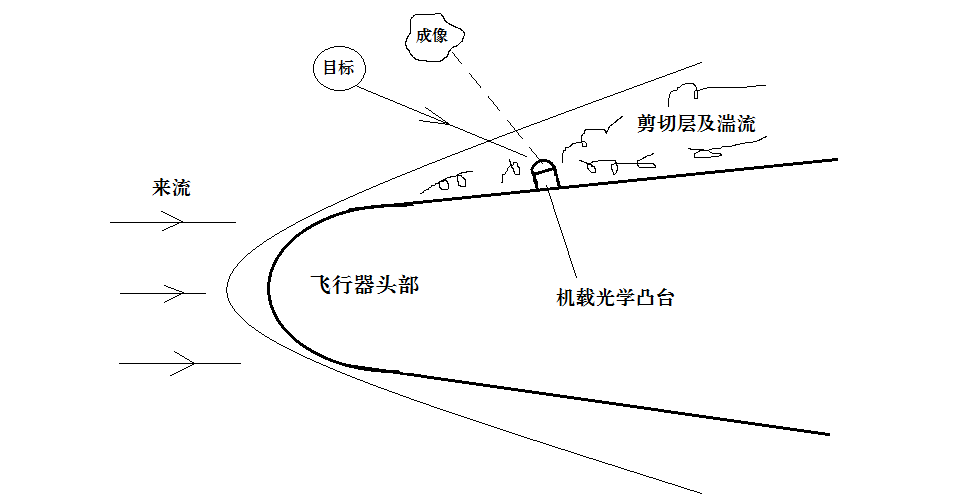
\includegraphics[width=0.8\linewidth]{aerooptic.png}
\caption{气动光学效应示意图}
\label{fig:aero}
\end{figure}

飞行器的速度越快,气动光学效应越明显,成像质量越差,制导精度越低,通过对气动光学效应的机理研究,可以深入分析可压缩流场对光波传输和光学成像的影响,以及研究如何对流场的物理参量进行控制,从而减少这些影响,提高成像质量及跟踪瞄准精度。

飞行器上一般会装备光学凹窗或者凸台来进行目标探测跟踪,由于凸台位于飞行器外侧,信号接收范围较广,因此在飞行器上采用机载凸台光学设备,能够有效扩大目标探测及主动观察寻的范围,同时凸台周围由于受到飞行器前部壁面导致的剪切流影响,并且容易形成二次剪切,这种情况导致凸台周围的流场较为复杂,对光传输影响较大,因此需要对机载凸台周围的流场产生的气动光学效应进行详细研究,从而为精确制导及目标跟踪提供有力支撑。

\section{气动光学的研究进展}
\subsection{气动光学理论的研究进程}
对于湍流的研究可以追溯到1883年,通过将染料喷射到壁面光滑透明的圆管内流体中的实验,英国物理学家Reynolds首次系统地研究层流向湍流的转换过程,发现了两种运动状态具有本质区别并确定了发生条件,他发表于1894年的文章中提出了今后被称为Reynolds数的无量纲参数,当雷诺数大于一个临界值时,流体的扰动不论多小,都将形成剧烈且随机的非常规运动,从而形成湍流\cite{renolds1894}。

而关于湍流对光学传输的影响的研究则要等到1952年,Liepmann采用纹影系统,分析了准直光束通过湍流流场产生的光学像差,首次定性地分析了气动光学像差,并且引入了对气动光学十分重要的均方偏差角的概念\cite{liepman1952}。
并且Baskins和Hamilton也在1952年对超声速湍流流场进行了试验,分析了光波在流场中的传播规律\cite{baskins1952}。

Stine等人于1956年成功地实现了焦平面上对时间平均辐射场的光学测量,他们主要利用初始平面光波通过针孔$(\Phi0.02\text{mm}\sim\Phi0.8\text{mm})$的方法进行测量\cite{stine1956},验证了Liepmann提出的偏差角公式,分析了流场中的电磁波散射情况,并且在参考前人工作的基础之上作了相对成熟的湍流场中的散射情况研究\cite{tatarski1961,villars1954,booker1950},Stine等人的工作为采用光学测量的研究方法来推演湍流的涡旋尺度提供了一定的参考价值,并且这种通过光学的信号测量来反向推测流场尺度特征的方法在今后成为了研究气动光学效应的一种重要研究手段。
 
G.W.Sutton在1969年的研究报告从理论上研究了湍流产生的折射率脉动对光束传播的影响,并且建立了基于物理光学的研究气动光学效应的数值模拟模拟方法,第一次提出相位变化作为评价指标,将远场成像的光斑光强分布情况和近场的波面畸变联系在一起,同时耦合了湍流对光强的衰减系数、相位均方差等,为今后的理论研究打下了夯实的基础\cite{sutton1969},Sutton的工作对于气动光学的研究具有里程碑式的意义,在1985年,他再次作了相关内容的报告,总结了之前关于气动光学的研究主要处于光学试验测量方法的研究阶段,指出下一个阶段的研究应该将重点放在具有实用价值的光学凹窗或凸台附近湍流流场的气动光学研究上\cite{sutton1985}。
 
美国航空航天局于1982年发表的综述\cite{gilbert1982}性文章比较详细地介绍了一些气动光学相关研究方法,包括基于时间平均流场的光波相位畸变$\sigma^2_\Phi$的数值计算方法以及一些比较基本的光学测量手段,比如阴影法和干涉法等直接测量方法,同时也介绍了使用间接测量的方法测量流场的速度以及流场密度,指出了对边界层研究的重要性\cite{trollinger1982}。

二十世纪九十年代,人们进行了很多对相位变化进行计算的理论模型,对斯特列尔比及光学传递函数等光场计算手段进行了研究,气动光学的动态测量技术在这个时期得到了迅速发展,华盛顿大学的Y.P.Tsai和W.H.Christiansent在1990年发表的文章指出了改善气动光学效应的方法,他们主要采用二维的欧拉方程来研究分析光束经过流场的剪切层时的传输特性\cite{tsai1990},并且这一结论的正确性得到了华盛顿大学的Larry Chew和WalterChristiansent的具体实验论证\cite{larry1990},证明了欧拉方程分析方法的可行性。

圣母大学的 Eric J. Jumper 和 Ronald J. Hugo在1995年成功地采用小孔径光束技术量化地测量了光波的波前畸变,这项技术是基于Malley探针的基础上实现的,文中指出这种方法可以用来评价湍流对气动光学效应的影响\cite{jumper1995},次年,两人发表了关于该项技术深度分析的论文\cite{hugo1996},文中指明这种测量方法可以用于测量湍流随机脉动的频率、当地速度以及湍流的脉动尺度等,他们积极地推广了小孔径光束测量技术,并且在此之后圣母大学通过这项技术在气动光学的研究中发挥了积极的作用, 2000年,两人再度合作发表的论文中构建了通过折射率场计算光波相位差的简化方程,并且该方程的可靠性已经经过了具体试验的验证\cite{hugo2000}。

在二十一世纪初期,关于气动光学理论的研究主要集中在具体湍流流场的机理研究以及光学方面的理论研究、测量方法上,美国圣母大学的Jumper与波音公司的Fitzgeraldb 两人合作完成了在这个时期的一项里程碑似的工作,他们发表的文章\cite{jumper2001}对该时期气动光学研究的特点进行了详细综述,文中主要介绍了气动光学研究的实验和测量技术的方法以及在实际应用领域中的发展情况,并且回顾了启动光学研究至今的发展历程,预测了在不远的将来,飞行器上将会装载高效可用的光学探测设备。 

Michael在2010年成功地利用高阶抛物方程近似求解气动光学效应,文中证明出采用四阶龙格-库塔配合第二阶的方法求解时拥有很高的精度,并且可以用高阶拉格朗日插值再度提高准确性\cite{michael2010},并且文中发现波长较短的光束在通过湍流区域时拥有更好的聚拢性,在计算中使用短波也更加精确。

Meng Wang等人在2012年的文章再次系统性地回顾了关于湍流介质引起的光学畸变现象的研究,重点介绍了气动光学的数值计算预测和物理机制\cite{meng2012}。文中提出,经过一系列流场包括湍流边界层、分离剪切层和光学设备周围的湍流的研究,通过数值模拟和实验研究,对这些现象有了一些新的物理理解。指出目前的核心问题在于可压缩湍流有较大的不确定性,并且大多数研究停留在亚音速阶段,提出需要更加精确的实验和计算技术来预测湍流运动,并简要讨论了削弱气动光学效应的方法。

国外的科学家们对气动光学的理论研究已经比较深入,发展了多种计算模型并且对湍流的运动机理进行了比较成熟的理论分析,但是目前较多的研究停留于低音速阶段,对于超音速的流场研究较少,且计算精度有待提高。
\subsection{实验及数值模拟上的进展}
气动光学问题是由于高速飞行器周围流场对目标成像及制导的严重影响而提出的,因此,早期的研究热点大都是以工程实用为目的的试验研究,美国、俄罗斯等大国对此投入了大量的成本,成立了专门的研究机构并建立相应的试验场地和实验设备等以展开长期深入的研究,并且研发了很多针对气动光学效应的数值计算分析的软件,在削弱气动光学效应方面取得了重要进展。

由于气动光学效应主要是高速飞行的飞行器周围流场导致的,因此对于气动光学效应的实验研究需要基于高速流场来研究,目前来说主要可以通过风洞来模拟具体的流场情况,例如阿诺德工程发展中心(AEDC)建立的高超声速风洞,如图\ref{fig:fengdong},它主要用来从事气动光学机理的实验验证工作\cite{havener1992},在二十世纪末,该工程中心9号风洞就能够在6s内完成流场结构及其引起的波面畸变的同时测量。基于对高超声速飞行器周围流场的实验研究需求,美国在上世纪八十年代建立了国家高能激波风洞,该风洞的两套设备能够提供2至15马赫数的流体速度,并且在后期对其进行了改造,使之能够满足气动光学在试验上的验证研究工作\cite{claspan1990}。
\begin{figure}[bhtp]
\centering
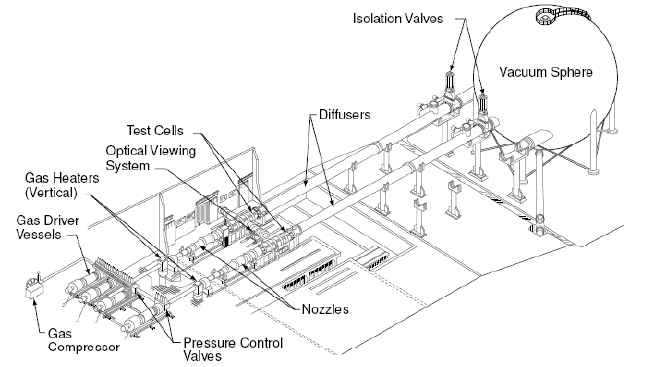
\includegraphics[width=0.9\linewidth]{fengdongshiyan.PNG}
\caption{阿诺德工程发展中心9号风洞机理图}
\label{fig:fengdong}
\end{figure}

近年来,气动光学的研究由大量的实验研究拓展到实验和数值模拟同时进行上,研究重点依然为气动光学效应机理研究以及对机载光学设备气动光学效应的控制。

Stanislav Gordeyev 和 Eric J. Jumper于2003年在实验中使用之前提出的小孔径光束技术研究了湍流边界层中的气动光学特性,实验研究的结果发现目标图像畸变程度与来流的速度的平方、来流密度以及湍流边界的层厚度存在正比例关系\cite{stanislav2003}。

Roberto C. Aguirre 和 Haris J. Catrakis在2004年为了分析当地尺度的波前特征,提出了一种气动光学波前各向异性参数的概念,并发展了基于该各向异性参数的气动光学评价方法\cite{aguirre2004},发现各向异性参数的可以用来衡量湍流引起的波前尺度的特性,当参数等于某一特定值时,光波波前在一定的小范围内拥有自仿射的特性。

Mani 和 Ali 等人在2005年采用大涡模拟的方法,研究了圆柱形的湍流流场对不同波长的光波产生的成像影响\cite{mani2005},发现波长较短的光束的远场成像主要受小涡旋影响。

John E. Pond 和 George W. Sutton在2006年采用三维流体运动方程组结合标准$k - $\textepsilon 湍流模型的数值计算方法,对三维凸台周围的流场进行了数值模拟,采用相位差和斯特列尔比两种参数对气动光学效应进行了评价,文中指出,可光学可调节的适应性系统虽然能够适当地减弱时间平均流场产生的气动光学效应,但是对脉动的湍流流场的矫正效果并不大\cite{john2006}。

Eric Tromeur 和 Eric Garnier在2006年为了求解光束通过流场时产生的相位差,采用了大涡模拟以及利用Sutton 模型分别与雷诺平均法和大涡模拟结合的三种方法对光束经过湍流流场后的相位变化进行求解\cite{tromeur2006},文中结果指出采用大涡模拟直接模拟流场,求解出的光学相位差有最高的精度,并且指出 Sutton的模型应用在非平衡边界层中时,求解得到的气动光学相位差有较大的误差。

2008年,Aaron P. Freeman 和 Haris J. Catrakis尝试了在湍流中注入不同频率的等离子体,证明了这种方法可以用来削弱气动光学效应\cite{freeman2008},成功地减少了27\%的光程差均方根。

Wyckham C 等人在2009年对流场产生的气动光学畸变进行了研究,主要将氦气射入从低音速到高超声速等不同速度的流场中,对光束经过其边界层后产生的光学畸变进行对比,得出了光学畸变主要是由于流场中的大尺度结构决定的,从而证明了大孔径近似理论的正确性\cite{wyckham2006}。

气动光学效应的风洞实验条件比较苛刻,并且实验成本较高、研究周期较长,而随着计算机技术的飞速发展,采用理论模型对流场进行数值模拟已经成为可能,并且相对于风洞实验能够有效节省成本,同时可以对流场参数进行调节从而控制流场结构并多次重复模拟,因此采用数值模拟的方法研究气动光学效应可以快速准确地给出精确结果,经过多次模拟达到预期效果后可以通过风洞试验进行验证。
\section{国内研究现状} 
国内关于气动光学的研究起步比较晚,在二十世纪末,中国航天科工集团提出了气动光学研究是高速导弹发展的重要组成部分,自此,国内的气动光学研究主要以工程需求带动基础研究,
随后的几年时间中航天科工集团多次发表了相关文章,对于国内在气动光学问题的研究成果进行了详细介绍,大大推进了中国气动光学的研究。随后,国内对气动光学效应的理论及实验研究、数值模拟、校正方法等方面都有一定成就,尤其是殷兴良和李桂春两位学者的研究气动光学的专著,对中国研究超声速飞行器光学头罩周围湍流流场的气动光学效应有非常重要的指导作用\cite{deng2008}。

2003年,殷兴良先生撰写了中国国内第一部研究气动光学的专著《气动光学原理》,中国工程院院士并且身为我国光学事业奠基人的王大珩先生称赞这本专著是“建立了国内该领域研究的基础”,以及“标志着我国气动光学这门现代光学新分支学科的形成”\cite{yxl2003qdgxyl},该书分为三个篇章,分别为气动光学研究的数理基础、描述及矫正方法的探讨,总结概括了中国航天二院下属的气动光学课题研究组多年以来的研究成果,对国内学者关于气动光学方面的科研工作提供了重要帮助,促进了我国气动光学的发展。

2006年,李桂春的《气动光学》正式出版,这本书被中国科学院院士庄逢甘先生评价为“将带动相关学科跨越式发展,拓展学科的研究领域,对国民经济建设及现代化建设具有实际的工程应用价值”\cite{liguichun2006}。该书抓住了交叉学科的关键,深入讨论了光波在非均匀介质即气体折射率梯度场$(\nabla n)$和散射场$(\nabla^2 n)$中传输的基本原理,总结了风洞试验中的光学测量技术,填补了国内气动光学学科方面的空白,同样对中国的气动光学发展具有重要意义。

在国内气动光学研究初期,许多学者也发表了大量研究论文,对国内气动光学的研究做出了巨大贡献,例如
郭永洪、 沈忙作等人在1998年的论文中简要介绍了采用数值模拟研究超声速光学头罩气动光学效应的分析过程,分别讨论了平均、湍流流场的气动光学效应以及两者的合成气动光学效应的计算方法\cite{gyh1998}。
费锦东\cite{fjd1998}在1998年发表于红外与激光工程的文章首次指出,由于气动光学效应的存在,高速导弹的红外成像制导系统对于目标的成像清晰度大大降低,提出气动光学效应的校正对于高速导弹光学头罩的外型设计、提高制导的精度以及抗干扰能力具有重要的作用。
房建成,杨照华等在2004年的文章中基于折射率场分别对不同尺度的涡旋结构的光传输特性进行了模型的建立,文中主要利用光线追迹法建立大尺度模型,而用统计光学法建立小尺度涡结构的光学传输模型\cite{fjc2004}。

最近十年,国内关于气动光学的研究得到飞速发展,取得了非常不错的成绩\cite{xie2007}。殷兴良在2006年建立了流场光学的工程计算模型,描述了气动光学效应对光学探测系统影响的经验模型,通过数值仿真,分析了气动光学效应对光学探测系统的影响与飞行器的飞行参数、光学探测系统参数和探测器积分时间的关系\cite{yxl2006gsfxq}。
赵剡等人在2008年的两篇文章基于数值模拟建立了光传输模型对光程差与光程进行了处理,利用带像差的光学传递函数理论,研究了对图像复原的方法\cite{zhao2008,zhaoz2008}。
史可天等人在2010年使用瞄视误差、Strehl 比以及含能半径等光学参数描述了湍流流场引起的光学畸变,具体分析了不同飞行状态和光学参数对光传输的影响\cite{skt2010}。

李波在2011年提出了实现了高速流场的气动光学研究的数值模拟,提出从流场角度出发评估高速流场导致的气动光学性能的评价方法,并且完成了高速飞行器光学窗口的初步设计\cite{libo2011}。
冯定华等人在2012年在通过数值计算得到精确的流场物理参数的基础上,分析了凹腔剪切层的光学传输效应,发现气流的剪切层结构会使光线抖动从而导致波面畸变,从而减少了斯特列尔比,削弱光束强度,并且会导致图像的位移,降低制导精度\cite{fdh2012}。
徐博在2015年利用Matlab及Zemax仿真模拟了对基于随机并行梯度下降算法的像清晰化自适应光学系统,将形镜形状变化引起的光线偏折以及光学系统自身的像差纳入考虑范围,对波前畸变进行了光电校正\cite{xubo2015}。
 
国内关于气动光学的研究已经取得了一定的进展,李桂春以及殷兴良的两部专著对国内关于气动光学理论研究以及光学校正作出了巨大的贡献\cite{yang2009,li2011},并且最近十年的相关研究也取得了飞速突破,同时国内的研究大多是对于凹腔的气动光学进行研究,并且数值模拟方面主要集中于中低音速流场,关于超音速的流场气动光学研究较少。
\section{论文主要研究内容及论文组织架构}
本文的研究来源于航天科技创新基金(SAST201350),国内现阶段对于气动光学效应的研究大多数处于低音速至低超音速流场的阶段,并且光学窗口的研究类型主要为凹窗型的探测窗口,而随着飞行器飞行速度的迅速提升以及探测范围的需求增大,未来精确制导及目标探测领域将集中于高速流场,同时将会装载光学凸台进行大范围的精确探测,因此本文将对高速飞行器和光学凸台周围流场的气动光学效应进行研究,主要研究内容可以分为如下的流场运动和光学传输两大研究方面:

(1)基于流体力学理论,研究从亚音速到高超音速等不同速度下的流场运动机理,讨论流体运动方程组的求解模型以及数值模拟方法,建立有效的数值模拟流程,然后采用计算流体力学(CFD)软件分析高速飞行器及凸台周围流场的情况。

(2)基于物理光学、线性光学、波动光学以及统计光学的理论,对高速流场产生的气动光学效应的机理进行研究,分析流场对光束传输影响的计算方法和评价体系,基于流场数值模拟得到的结果,通过Mathematica数值计算,研究分析凸台光学窗口周围混合流场的气动光学效应。

本论文的组织结构如下:

第一章:说明了课题研究的背景,回顾了以往关于气动光学理论研究、实验测量以及数值模拟方面的成果,分析了研究特点以及存在的困难,提出研究凸台周围高速流场引起的气动光学效应的必要性。

第二章:介绍了流体运动的基本理论,分析了大涡模拟以及雷诺平均模拟两种气动光学的数值模拟方法,推导了基于$k-\varepsilon$模型和$k-\omega$模型的SST混合二方程模型,最后分析了高超声速流场的物理特性。

第三章:对高速流场模拟前需要的定解条件以及控制方程的离散作了相应设置及推导,建立了可压缩流场数值模拟的具体流程,最后通过ICEM建模软件建立了三维导弹、机载凸台的模型,使用Fluent基于$k-\omega$SST二方程模型对不同运行速度下导弹及凸台周围的流场分布进行了数值模拟及分析。

第四章:分析了光束在高速湍流场中的传输特性,基于光线追迹法、波动光学以及统计光学的方法对平均流场、湍流脉动流场分别分析,推演了偏移角、斯特列尔比以及光学传递函数等气动光学评价方法。

第五章:通过G-D系数建立密度与折射率的直接关系,讨论了高斯光束以及夫琅禾费衍射现象,最后基于CFD网格离散化求解方法,计算了不同速度、不同入射角下凸台光学窗口周围的波面畸变,对光学孔径内受湍流流场影响的斯特列尔比和光学传递函数作了计算,得到了高斯光束经过流场前后的光斑变化。
 
 第六章:对本论文的工作作了相应的总结,并且对该课题未来的进一步研究进行了展望。
 
 
 %--第一章--
%\chapter{电子商务与国际贸易}
\section{电子商务的基本概念}
电子商务,望文生义,即通过电子设备进行的商务贸易往来,广义地说,就是一切与电子、数字化处理相关的商务活动都可以认为是电子商务,重点在于商务活动发生于网络计算机环境;狭义地说,就是通过网络手段进行价值产品的买卖商务活动,比如网络购物。

电子商务的发展方便了很多人,解决了时间、空间的冲突、限制,人们可以在网上进行购买,人们可以利用碎片化的时间享受购物过程,如今利用淘宝、京东、拼多多的购物平台的消费者越来越多。并且随着移动设备的迅速发展,人们只携带一个手机就可以通过任意平台进行贸易往来,甚至一些社交网站也提供购物平台的入口,可见电子商务发展之迅速。

\section{电子商务的主要特点}
电子商务具备以下特点:
\begin{enumerate}[(1)]
\setlength{\itemsep}{0ex}
\item 合作性高,电子商务的整个流程可以看作是一个协调工作的过程,生产、运营、销售等都是不可或缺的环节,线上线下的支付、货物的运送等也都离不开银行、物流部门、通信中心、技术服务人员等相互默契的合作,协调完成,各环节都需要精密合作。
\item 通用性强,电子商务作为目前广受欢迎的经营方式,具有通用性,数字化的网络世界中的交互都是基于互联网的操作。
\item 高效快速,在电子商务环境下,互联网将整个地球纳入地球村,人们的工作已经不再受到时间、地点的限制,客户可以以非常简单的方式在短时间内完成以往复杂的业务活动,并且能够随时随地通过互联网查询交易、资金、等信息。
\item 便捷严谨,通过规范贸易规则,基于互联网平台发布交易模板,能够有效地规范交易流程、合约等,交易双方仅通过简单地填写模板就可以完成贸易,
而模板既可以简化交易,又可以排除人为地漏洞,提高系统的严谨性。
\item 安全手段多,任何时候,安全性是交易的重中之重,相比与传统手段,电子贸易由于是基于互联网的交易,
拥有各种安全系数高的保密手段,比如加密签名、权限控制等,但是同时由于互联网的高效便捷,一旦出现安全漏洞,损失也比较巨大,因此安全性需要作为电子贸易的第一考量。
\end{enumerate}

\section{国际贸易的基本概念}
国际贸易又称通商,是指跨越国境的货品和服务交易,也就是国与国之间的贸易往来,能够调节国内的生产要素利用率,改善国际之间的供求关系,调整经济结构,增加财政收入。国际可以发生在两个或多个国之间,一起完成一项贸易,国与国之间的物品、价值商品交换,进行经济交流,跨境贸易,一般的国贸可以分为加工贸易、商品贸易、服务贸易等。根据贸易量的参与国,可以分为双边贸易、多边贸易,双边贸易指两个国家之间的贸易,一国进口一国出口,无需其他多家参与,多边贸易指三个或三个以上的国家参与贸易,在现代全球化经济体制下,多边贸易的发生更为频繁。
\section{国际贸易的主要特点}
国际贸易本质上也是商品、货币等价值的交换,但是国际贸易与老百姓日常接触的贸易存在很大区别,比如交易范围更广,距离更远,涉及领域更多等等。总的来看,国际贸易主要有以下几个特点:
\vspace{-0.5ex}
\begin{enumerate}[(1)]
\setlength{\itemsep}{0ex}
\item 波动性大,国际贸易牵扯两国或多国经济,但国与国之间不仅仅是经济合作,还有国际形势影响,因此,容易受到外部政治环境、双边关系等影响,波动性大。
\item 条款量大,国际贸易的参与国可能采用不同的语言,同时,英语作为世界的通用语言也经常要参与条款内容,合同的签订等还需要考虑双方的宗教、习俗、政策、保险、仲裁协商、收发货等方方面面。
\item 体量巨大,国际贸易由于是跨境交易,参与双方运输等成本较高,提高了准入门槛,贸易量也因此上升,单次交易一般都是大宗交易,即便是普通消费网购,一般也由网络平台进行统一综合处理发货。
\end{enumerate}
\section{国际物流的基本概念}
以现代物流理念为理论依据,在全球范围内以国为划分单位,进行工作物流分工,建设物流设施,应用物流信息传递技术,提高物流工作效率,最大化提升物流速度。互联网解决了国际贸易的商品交易、货币支付等上层问题,而基层的货物运送则完成了国际贸易的最后一环,完善了整个电子商务的闭环,国际贸易得以展开,从而飞速发展。随着全球经济一体化的进步,市场经济愈加需要国际贸易的支持,国际物流的支撑与保障必不可少。
\section{国际物流的主要特点}
现代国际物流目前展现出以下几个特点:
\begin{enumerate}[(1)]
\setlength{\itemsep}{0ex}
\item 距离远成本高,国际贸易的货物运送可想而知,必然伴随着跨境运输,运送距离可达几千上万公里,路途遥远,势必要采用高效管理的方式保证长途运输的稳定。同时由于距离的原因,导致管理、运输等物流成本巨大。
\item 巨头化,跨境物流成本高,准入门槛也就相应提升,从而出现几家物流巨头相互竞争的趋势,外界资本也流会入各大巨头而不是另起炉灶。
\item 外包化,物流成本的巨额费让许多企业放弃自己运输货物的方式,将物流外包给专业的物流公司,转而将更多的资金投入研发或者增值服务。
\end{enumerate}

\section{本章小结}
本章主要介绍了电子商务、国际贸易的基本概念以及两者的主要特点,同时简单介绍了在国际贸易中扮演重要角色的国际物流的概念及特点,现代国际物流可以说是国际贸易的桥梁,补全了电子商务的重要环节,增强了市场活性,完善了电子商务的贸易模式,推动了国际贸易的发展。
%--第二章--
%\chapter{电子商务对国际贸易的影响}
电子商务依托于强大的互联网技术,几乎改变了国际贸易的整体构成及贸易方式,冲击着传统贸易,重新定义了国际贸易。随着电子商务的愈加成熟,国际贸易的经营主体以及贸易方式都发生了显著变化:

国际贸易的贸易主体发生了重大变化,
以往的贸易往来主体通过中介进行买卖服务或者担保,而如今只需要通过成熟的网络平台,比如阿里巴巴等B2B平台进行直接交流,省去了中间商,同时买卖双方通过交易平台能够快速定位所需客户。这种贸易模式依托于网络平台公司在其专业领域的领先技术,完成单个公司无法实现的市场功能,进行信息整合推送,承担着信息搜集、处理、传递、推荐功能,完成了企业间的弱联系,改变了以往企业间的贸易模式。

国际贸易的市场交易模式发生了重大变革,
传统市场存在的前提条件是空间上必须有一定的地域,聚集各个商家进行贸易往来,而电子商务另辟蹊径,利用互联网的虚拟特性,以全球的信息网为基础,将全球贸易笼络成一个超级市场,促进了世界经济的全球化,改变了国际贸易市场。

\section{电子商务的积极影响}
电子商务大大压低了国际贸易的贸易成本,电子商务依托于国际互联网,交易双方通过网络即可完成交易,节约了时间成本,而物流的出现



现代信息技术大大降低了国际贸易的经营成本。以国际互联网为核心的电子商务应用不在以时空为界限,电子商务的整合效应也简化了业务的流程,网络第三方服务也日益完美。网上订货、网上促销、网上谈判、跨国公司内部网络销售均为电子商务交易开辟了新形式。信息技术与社会化服务系统结合产生了EDI工程,进出口商利用电子表格进行商品的报关、商检、保险、运输投保和结汇等工作。这种做法大大减少了人才、物力和时间消耗,降低了流通成本和交易费用,减少了中间环节,加快了国际贸易的节奏。


  电子商务突破了时空限制,贸易服务的供应者不必跨出国门甚至家门就能为别的国家的客户提供各种服务。另外,公司足不出户就可以同时接到来自不同国家的业务,而不必担心日程安排和国际旅费等方面的问题。例如:在新产品开发、工业设计、咨询人才培训、医疗诊断等领域,这种扩大的服务需求直接导致国际服务贸易的飞快发展,促进国际贸易商品结构的高端化。

  4.
  1.电子技术层面,应采用一系列行之有效的电子技术方法,并保证交易业务的安全。目前,最普遍的方法有:应用数字时间解决电子交易文件发出的时间认证问题;应用数字证书解决网上交易对象身份认定问题;应用非对称密钥密码技术解决交易信息传输过程中的保密问题;应用数字摘要、数字信封、数字签名等方法解决交易信息传达后的完整、正确、未被修改的验证问题。
  
    2.加强法律法规的研究与制定。现行国际贸易法是基于传统的有纸贸易方式而制定的,所以许多法规不适用于电子商务贸易方式,对电子商务的发展会带来许多难以克服的障碍。为了保证电子商务的良好发展,围绕电子商务发展及相关的信息安全、网络管理、知识产权保护、金融结算、等问题,应加快现行法律法规的修改步伐,及时制
  
    定、出台新的贸易法规。
  
    3.降低过高的资费,改革收费制度。制约电子商务在我国发展的一个重要原因就是高收费。例如:网费,目前我国国内互联网的上网费用比美国高出14倍,国际专线价格更加昂贵,DDN专线不但收取月基本费用,同时收取流量费。改革现行收费制度,建立一个完善的符合市场要求的收费体系,下降过高的资费能有效提高我国公民对电子商务的接受水平,是促进我国电子商务发展的重要条件。
  
    4.建立人性化的国际CRM系统。CRM的核心思想是了解客户所想,满足客户所想,从而提高企业经营绩效。在外贸企业中建立CRM,不但能有效避免传统贸易手段中对业务员的过度依赖,而且能更加高效、方便、快速地实现与前端客户的交互,满足客户服务。
  
    5.积极参与国际合作与对话。对于国际性讨论对话活动,我国政府虽有参与,但不够积极。实际上,这些对话活动不但决定不同国家、地域之间的利益分配,直接影响着电子商务下新交易法律法规的制定,而且加强了世界各国的交流,提高了各国电子商务的国际兼容性。对此,我国政府应予以足够重视。
  
    四、结论
  
    电子商务时代瞬息万变,国际贸易展现出的变化是对新的贸易方式和贸易环境的变现。根据专家评测,20140年全球电子商务交易额将达到一万亿美元。中国作为最大的发展中国家,正面临着应用电子商务促进国内经济发展,正是走向世界的机遇也是挑战。想要更加有效地参加国际市场竞争和在经济全球化过程中获得最大的利益收货。我们应当把电子商务在国际贸易中的姿态放在首位并且借鉴发达国家的经验,培育我国公司在国际贸易中应用电子商务的竞争能力,这将使我国国际贸易发展创建一个新的里程碑。
\section{电子商务存在的问题}

(一)电子商务的积极影响

自从在国际贸易运用了电子商务,国际贸易的复杂流程变得非常简便。相比于传统的国际贸易,如果国际贸易非常频繁,就会使得国际贸易间的手续流程非常繁杂,耽误了很多的时间,存在很多的误差之处,贸易效率低。而随着电子商务的使用,国际贸易立刻发生巨变,因为电子商务是一种无纸交易,把传统贸易模式下的复杂琐屑过程变得非常快捷,得到很多国家的重视。无纸交易是指在现代信息技术的帮助下,通过互联网的快速传播,使得双方的交易信息迅速传达至对方,这样一来就可以减少传统贸易间的订单需求等,快速的达成贸易目的。无纸交易的主要核心是电子数据间的交换,简称EDI,EDI是指利用计算机技术和互联网的方便特点简化国际贸易的业务流程。和传统贸易相比,不需要前期的贸易准备、中期的贸易技术管理人员洽谈和最后贸易订单签订和人员跟进等。因此使用电子商务可以大大减少订单的各种准备工作,提高贸易的效率,同时又除去了不必要的成本投入。

(二)电子商务的消极影响

电子商务带来方便的同时,不可避免也造成了一些消极的影响。首先电子商务加剧了发达国家与不发达国家之间的差距,因为电子商务使用的基础取决于高度发达的电子信息技术和互联网技术等先进的科技技术,而电子商务的快速使用又使得国家间的贸易业务变得更为广阔,加速了国际贸易的发展,提高了国际贸易的效率。因此在这种不公平的发展基础上,发达国家比不发达国家更有优势,发达国家与发展中国家的差距将会越来越大,出现马太效应。其次,相比较于传统的贸易模式,电子商务主导的贸易模式极易造成大量的税款流失。因为电子商务的快速发展,造成了大量贸易的无纸交易,虽然可以加快贸易的效率,但不可否认也在一定程度上影响了发展中国家的税收,导致发展中国家的发展滞后。由于互联网虚拟的特点,很容易使得无纸交易变成欺诈交易,造成国际贸易的混乱,影响国家的正常收税活动,同时由于电子商务的无纸交易,导致了国内中介的衰败,影响国家税收。 




电子商务管理方式在国际贸易经营管理方式中的变化逐渐加大,交互方式网络运行机制对于电子商务而言,其变化程度极其深远,在此种发展背景之下,国际贸易中能够所展现出的最优化配置,借助国际贸易世界经济来完成,此时,若是从全球化角度进行分析,市场机制效能才完美彰显。老旧式贸易模式现在被此种贸易形势替代掉,四流一体成为主流,简而言之,就是将物流作为支撑,将资金流视为基本运作形势,商品流通是主体,创新整改后的经营管理模式特性正是如此,此种经营模式在实施商业贸易交流时将信息网络作为依据,并且站在不同角度之上实施真正意义上的互动。我们应该意识到,网络可以使生产者和用户以及消费者之间实现互动,供货制度和零库存生产,二者才能得以完美实现,商品流动性就会变得更加的符合市场规律,与社会需求相互契合,符合经济发展诉求,中间商就是我们所熟知的信息网络。

三、现存问题要点分析

电子商务若想得到长远发展与立足,应该借助信息基础建设来完成目标,但是现有信息基础设施建设还有待增强,并且此时的网络规模局限性十分明显。重要的网络安全问题没有透彻得到解决,网络对于电子商务而言,十分重要,网络数据传递、网络数据交换如此,安全性处理亦如是。商业交易在网络上进行,安全性未能得到透彻保障,当前我国经济出在转型时期,尚未形成较为成熟的市场,社会信用结构体系没有得到透彻完善,网络交易受影响因素主要涵盖了身份识别内容、商业机密内容和通讯安全内容,尤其是没有授权的信息非法篡改和信息内容恶意拦截,网络交易和客户信息记录保存等仍有些许漏洞。电子商务对老旧式商业法律和商业习惯造成冲击,老旧式商事立法和商事习惯中,有纸式模式成为主流,但是电子商务过度的去依赖网络空间,理解为不完全在纸张基础上进行交易,因此若是站在客观角度进行研究,老旧式立法办法和电子商务运作间从根本上讲没有联系。但是电子商务这一事项上所涉法律事务繁多,风险仍在,那么电子商务在具体应用阶段就会滋生诸多障碍因素。虽然当前网络信息和电子商务在我国有了法律条文规定,但权威性法律甚是匮乏,争端出现其实没有透彻解决的可能,这样一来,电子商务发展稳定性和电子商务发展快速性,二者都会受到影响。

四、解决办法分析

(一)顺势而为

全球经济一体化进程日渐加快的今天,国际贸易领域范围内,信息技术应用频率有所加快,世界上每个国家在发展商务的整个阶段内,电子商务都发挥着巨大效能,我国若想在本世纪竞争中独占鳌头,就必须将电子商务作为核心研究对象,只有这样,才能在一定程度上与发达国家“抗衡”且具备一同进步和发展的机会。

(二)依法而行

电脑空间法律实际上是世界性的,本世纪中国国际贸易是一个发展快速的阶段与过程,自身具备发展前景,电子商务此时就必须做出改变,国际贸易竞争也要向发达国家看齐,与国际立法去向靠拢,并立足于国际立法标准。电子商务发展,务必要与法律之间达成匹配,按照电子商务发展基本需求,立法部门应该强化电子提单管理力度和司法官权的强化力度,对合同法和票据法以及消费者权益保护法进行健全,在安全认证方面务必加大规范力度,在线支付与电子商务机构和企业管理方面也要重视起来,不同类型的电子商务贸易都要透彻规范和整改。

(三)由浅入深

基础建设要做到位,为电子商务发展提供强劲的物质基础支持,国家方面电子商务现在已经得到了大量影响,信息基础设施建设优良决定着机会和空间的发展效果,所以为了促进电子商务更好更优的发展,我们应该注重信息基础设施建设,与此同时,提升网络资源利用效率,长此以往,行业分割管理制度会愈加完善,体制日渐健全,资源效益会得到质的提升。中国经济发展,电子商务方面会受到过高收费限制。

五、结束语

今后国家贸易发展,电子商务在其中起到了至关重要的效能,外贸企业务必要坚持自身原则,提升竞争力才是根本,要对电子商务进行深度认知,建立站点,供求信息扩大,建立客户群和交流渠道,树立优质企业形象,在国家贸易中利用电子商务手段谋求更为广阔的天地。 



 
 
 

3 现代物流对我国对外贸易的促进作用

3.1 降低了经营成本

现代物流行业的发展,对我国对外贸易活动的开展具有极强的促进作用。最直接地体现在降低了经营的成本。一般而言,要想提升贸易效益,首先应该综合考虑各国在经济方面所具有的优势。而优势则体现在对成本的控制与比较方面。但针对目前国际贸易发展现状分析,经济的高速发展使得成本降低的空间越来越小,可是在物流方面可以压缩的空间却越来越大。相关数据表明,我国物流行业及其相关行业一年的总支出大约为19000亿元,而物流经济效益在我国GDP总量中所占比重高达25%。故而,通过物流活动中各个环节的协调,可以使物流行业的经营成本不断降低,从而降低国际贸易成本,提升国际贸易效益与水平。

3.2 扩大了贸易规模

现代物流的发展也使得国际贸易的规模不断扩大,因为目前我国的对外贸易伙伴处于相对集中的状态,且大多为欧亚以及美洲国家。这足以看出我国对国际贸易的依赖程度相当高,不利于将市场扩展。而现代物流的发展则对国际贸易的规模有重要影响,尤其是现代物流发展中,口岸物流的建设以及交通运输网络的完善、电子信息技术的进步等,都为我国国际贸易活动的开展以及货品的运输提供了条件,从而扩大了我国国际贸易的整体规模。

3.3 加快市场反应速度的同时也提升了整个市场竞争力

我国市场中的商品普遍存在技术含量较低、劳动力投入较大的特点。也正是因为我国这种传统的产品生产形式,我国的产品对外竞争力较弱。为了有效改善这种现象,不仅需要增加产品的研发力度,另外还需要通过科学有效的管理,加快进出口企业对市场的反应速度。既需要降低交易成本,还需要生产适销对路、技术含量较高的产品,实现我国进出口经济的协调发展,从而提供较好的产销服务,提升我国产品在国际贸易竞争中的竞争实力。

探究现代物流对国际贸易的促进作用,实际上也是实现我国现代物流发展、促进我国国际贸易进步的重要举措。要想转变为贸易大国,现代物流企业在其中的重要性不言而喻。不仅需要从多方面进行改变,同时还需要历经长时间的付出。作为现代物流企业,要明确与国际贸易之间彼此的促进作用,这样将有利于实现现代物流对国际贸易的推动作用。

4 我国现代物流行业发展的对策

4.1 转变观念与意识,提高服务质量

作为现代物流企业,必须对传统的物流服务方式与手段进行创新。物流企业因为规模较小,所以往往缺乏相应的竞争实力。故而需要我国物流企业的领导人员转变自身的意识与观念,从而不断提升自身企业的服务质量。既需要为货主提供高效率的物流服务,还需要具有个性化服务特点,满足客户个性化的消费需要与服务需要。

4.2 加快现代物流基础设施建设

目前我国物流基础设施建设还相对落后,与国际贸易中需要实现的物流机械化、装备现代化要求较远。所以要想更好地发展我国现代物流行业,并且使之与国际贸易发展相契合,加大物流基础设施建设刻不容缓。比如可以建设集装箱专用码头,这是现代物流行业发展的基础。同时更应该满足国际物流连续性作业的要求,引进众多国外先进技术,实现物流设备的引进、研制、发展,从而提高货物的运输效率与水平。

4.3 培养专业物流人才

培养专业物流人才,是我国现代物流行业在未来的发展过程当中重要的基础和保障。所以许多院校也可以开设物流相关课程,其目的就是为物流行业提供更多既具有较强理论性,又具有极强操作性的专业人才。不仅需要大力引进国内外优秀人才,还需要建立起相应的培训与奖励制度,通过众多的方式留住优秀人才,进而实现我国现代物流企业的长久进步,为我国国际贸易的发展带来基础性帮助。

4.4 政府和国家给予足够的扶持与支持

政府和国家的支持,是现代物流企业发展的重要保障。尤其我国现代物流行业发展还处于初步发展阶段,所以往往需要国家的支持,这样才能规范我国的贸易市场,实行严格的进出口原则,从而让现代物流企业为国际贸易发展服务。

5 结 论

现代物流行业在未来的发展中,必将呈现出蓬勃发展的态势,同时其自身对国际贸易的影响也将越来越大。因此,现代物流企业必须通过合理的方式对自身进行创新与完善,制定出与国际贸易发展和市场经济相适应的对策,从而为世界贸易的繁荣与进步提供基础与条件。













全球经济一体化的发展与互联网科技的发展,让国际贸易变得越来越频繁,贸易对经济发展的推动作用是显而易见的。我国在受到2008年全球经济危机的冲击之后,国际贸易的总体水平稳中有升,为我国的出口贸易企业提供了良好的发展机遇,并取得了非常不错的成绩。但我们仍然需要牢记古人“居安思危”的思想,我们在看到成绩的同时也要看到风险存在,并对这些风险采取一定的规避措施,在风险真的来临时,能够把企业的损失降到最低。

一、国际贸易风险的类型

(一)政策风险

政策风险,主要是指随着全球贸易增多而使贸易摩擦不断地加剧。在国际贸易中,反倾销案件持续增加,技术性贸易壁垒也普遍存在。这让全球的贸易关系也变得越来越复杂:一方面,全球经济一体化的发展让全球贸易趋势呈自由化的方向发展;另一方面,在世界贸易组织的框架内,区域经济的合作获得迅速的发展,各种排他性的贸易保护主义开始不断地以各种看似合理的方式出现。关税是一种保护本国市场发展的贸易壁垒被普遍地使用和接受,变得越来越透明,但是技术性的贸易壁垒,却在一些发达国家出现,将其他国家的竞争企业排除到国门之外。

(二)操作风险

操作风险,主要是指对国际通用的贸易惯例和贸易术语了解的不足。贸易术语很多时候是一种惯例,明确了参与国际贸易各方的权利与义务,如果参与贸易的一方对这些术语不熟悉,就会在贸易中出现操作上的不合规矩。并且一旦被国外的不法商人所利用,就会产生意料之外的贸易纠纷,最严重的就是导致惨重的经济损失。所以,合理地对贸易进行了解和操作十分重要。

(三)汇率风险

国际贸易之间的结算并不像国内贸易一样都使用人民币。那么,不同币种之间进行清算时就存在一个本币与外币的折算比率问题。但比率并不是固定不变的,而是随着国际外汇市场出现波动而有所浮动,这就造成了国际贸易企业各方的实际收入与当初预想的会有不同(贸易中的汇率风险),进而导致外贸企业净利润的增加或者减少。采取一定的措施切实地对外汇风险进行防范,是外贸出口企业必须要重视的问题。

二、国际贸易风险管理的原则

国际贸易中的风险规避管理是在一定原则的指导下进行的,笔者将这些原则总结如下:

(一)风险回避原则

每个外贸企业都有自己独特的产品和擅长领域,风险回避原则就是指出口企业不涉及那些自己不擅长的领域,或者是预测到可能会出现风险的领域。虽然在这种原则的指导下可能会使企业错过一些获得高收益的机会,但是只有采取这种措施才有可能规避较大的风险。

(二)风险抑制原则

风险抑制原则,是指企业通过采取有效的措施对风险进行监控,在风险成形之前就将其扼杀。在对汇率风险进行防范时,风险抑制这个原则是非常适用的,因为很多时候汇率的变化之快,不会给企业留有反应的时间来采取措施挽回损失的。

(三)风险转移原则

参加国际贸易的企业可以通过购买商业贸易保险等方式,将可能产生的风险转移给第三方,这就是风险转移原则。这需要企业的管理者对风险有足够的认识和了解,以便采取合适的投保或者其他转移方式。

三、规避国际贸易风险的有效措施

通过前文对国际贸易风险类型的分析和风险管理的原则,笔者提出了以下对国际贸易风险进行规避的措施:

(一)对贸易伙伴的信用情况进行严查

贸易双方的相互信任和了解是国际贸易中非常重要的一环。为了增进这种信任和了解,为了能够找到信用优质的合作伙伴,需要我们的企业在双方进行合作签字之前就对对方的企业进行严格的调查。这是贸易合作准备工作的一部分,调查的途径主要是通过委托专业的咨询企业进行调查咨询,或者借助银行代理系统对贸易伙伴的信用情况进行调查。

(二)国家加大对人民币汇率的调控力度

关于人民币的汇率都是依据国家的国情进行制定的,常常使用的就是固定利率,但是在国际市场的贸易中,结算方式是双方互相协商的结果。所以,为了我国的企业在协商时有更多的资本,在制定人民币汇率时,就要考虑到具体的国情和人们的利益,尽量地保持汇率的稳定。一些强势的经济体国家会利用国际货币体系来转嫁本国的经济危机,从而得到更多的经济利益。这是我国需要坚决抵制的,尤其是要反对他国使用强制性的手段迫使我国利率的提升。

(三)运用技术手段切实转移风险

在国际贸易进行的过程中,我国的外贸企业可以根据风险管理的原则,使用一些技术手段来有效地规避风险。第一,可以通过合理的投保来降低运输风险。因为国际贸易的路途通常非常遥远,且耗时较长,在整个过程中存在着大量的隐患和风险,如海盗、战争、空难等,企业需要通过办理运输保险来促进企业外贸事业的发展。第二,可以通过妥善地利用国家提供的出口信用保险。这是由国家成立的专门的保险机构来向出口企业提供的一种政策性的保险,承担一些商业保险不愿意承担的保险业务,能够有效地规避贸易中的各种风险。第三,通过积极地引入国际保险业务来提供综合性的财务服务,规避外贸过程中收汇风险等。

(四)遵循国际贸易惯例

国际贸易的惯例通,常是指国际性的贸易组织或者商业社会的团体制定出来的一些贸易准备、规矩。这需要参与国际贸易企业的工作者牢牢地掌握,以便企业在签合同、交货物、结货款时能够严格地按照进出口贸易的规则程序来办事。妥善地处理好合同、单据、货物之间的关系,特别要注重信用证与单据之间的关系,以确保货款能够得到及时的清偿。同时,对国际贸易中的贸易术语进行全面的了解,以免在进行国际贸易的过程中因为不了解而遭受损失,面临“哑巴吃黄连,有苦说不出”的无奈局面。

四、结束语

国际贸易是一项对外部环境有较高依赖性的贸易活动,国家之间的各种关系的变化、政策的变动都能引发国际贸易的动荡。尤其是随着国际市场竞争激烈程度的加剧,各国之间为了本国经济的发展和贸易的顺利进行会出台各种办法,这些因素都让国际贸易变得更加的复杂、多变,导致贸易风险、贸易摩擦事件的频繁发生,并造成了一定损失。但凡事皆有两面性,如果我国的外贸企业能够抓住机遇,积极地进行国际市场的开拓,采取有效的措施来规避风险,那么我国的国际贸易一定会发展得越来越好。%--第三章--
%\chapter{非均匀流场中的光传输特性研究}
光是一种电磁波,物理学中存在大量关于电磁波在介质中传播特性的研究,这些研究表明光在介质中的传播过程呈现较强的波动性,麦克斯韦的衍射理论正是研究光波的传播的非常有利的工具,以场论为基础,建立电磁场中电场、磁场的微分关系,经过简化消元后,能够推导出非均匀介质中光传播的波动方程,如式\eqref{eq:maxwell}所示。
\begin{equation}
\begin{cases}
\nabla^2\mathbf{E}-\dfrac{\varepsilon\mu}{c^2}\cdot\dfrac{\partial^2\mathbf{E}}{\partial t^2}+\dfrac{\nabla\mu}{\mu}(\nabla\times\mathbf{E})+\nabla\big[\mathbf{E}\cdot\dfrac{\nabla\varepsilon}{\varepsilon}\big]=0\\
\nabla^2\mathbf{H}-\dfrac{\varepsilon\mu}{c^2}\cdot\dfrac{\partial^2\mathbf{H}}{\partial t^2}+\dfrac{\nabla\varepsilon}{\varepsilon}(\nabla\times\mathbf{H})+\nabla\big[\mathbf{H}\cdot\dfrac{\nabla\mu}{\mu}\big]=0
\end{cases}
\label{eq:maxwell}
\end{equation}
式中,$c=3\times10^8m/s$是真空中光速,为,$\mathbf{E},\mathbf{H}$为电磁场的电场及磁场,$\varepsilon,\mu$为相对介电常数及相对磁导率,绝大多数物质的介电常数$\varepsilon>1$,而对一般气体来说,相对磁导率$\mu=1$。

假设光在介质中的传播速度为$v$,那么物质的折射率$n$是由光在真空中与介质中的速度之比来定义的,即$n=c/v$。而光在介质中的传播速度又与该介质的相对磁导率、相对介电常数有简单关系:$v=c/\sqrt{\varepsilon\cdot\mu}$。联立两式,可以很快得到折射率与相对磁导率、相对介电常数的关系:
\begin{equation}
n=\sqrt{\varepsilon\cdot\mu}
\end{equation}

在研究湍流的气动光学效应时,流场的折射率$n$是与位置有关的函数,如果考虑通过流场的光波是波长为$\lambda$单色波,并且波函数$\mathbf{U}$与时间有$exp(-jwt)$的依赖关系,$w$为频率,由于流场的尺度$\Lambda$远远大于波长$\lambda$,可以将后两个偏振项近似为0,对方程\eqref{eq:maxwell}进行化简,可以得到简洁的波动方程:
\begin{equation}
\nabla^2\mathbf{U}-\frac{n^2}{c^2}\cdot\frac{\partial^2\mathbf{U}}{\partial t^2}=0
\label{eq:guangbodong}
\end{equation}
式中,$\mathbf{U}$是光波矢量,$n$为折射率。

对方程\eqref{eq:guangbodong}描述了光波在介质中的传输过程,对方程的求解能够精确描述流场对光传输的影响,但是波动方程很难得到解析解,并且由于飞行器周围流场由层流及湍流构成,流场结构非常复杂,使折射率随机变化,大大加大方程求解难度,目前工程上对气动光学效应研究的方法一般可以分为光线追迹方法、物理光学方法、波动光学方法以及统计光学方法这四类\cite{sutton1994}。

光线追迹方法主要是通过光线折射的原理,对从目标发出的每一条光线进行追踪,由不同光线在像平面的形成的点集合可以得到流场对光波传输的影响,该方法简单易行,但是由于采用了几何光学近似方法,无法确定传输特性与波长的关系,不能给出流场对光学传输特性的全面描述。

物理光学方法首先计算光波通过流场后的相位差分布,对其进行傅里叶变换求解相平面振幅分布,从而可以反推出流场的点扩散函数及调制传递函数,因此只要求解出光瞳函数,物理光学方法能比较全面地给出流场对光传输的影响。

波动光学的方法主要是利用子波原理,按照整体波面传播,计算传输到下一波面的过程,可以离散求解,最后得到波面像差,计算精度很高,但是折射率的随机分布使计算过程非常复杂,目前难以解决。

统计光学法将流场的变化看成具有一定特征的随机过程,利用概率论及随机过程结合实验数据,统计分析光波在流场中的传播特性,该方法可用于计算湍流脉动部分对光传输的影响。

实际工程共可以结合这几种研究方法进行综合考虑,将层流流场看作不随时间变化的非均匀流场,可以通过光线追迹及物理光学方法来求解层流流场的光传输特性,而对于具有随机性的湍流流场,可以引入流场“冻结”概念,对不同时刻的流场使用统计光学方法来描述。
\section{光线追迹理论及方法}
由于光在传输过程中呈现较强的波动性,导致在通过尺寸较小的空隙时会产生衍射现象,但是如果波长$\lambda$无限趋近于0,就消除了衍射情况,可以认为将光分为了无限多的细光线,光线就确定了光的能量传输走向,而在通常情况下,光学仪器尺寸远远大于光波长,这时可以忽略波长,光线追迹理论就是基于此假设。本文研究的光传输距离较短,且流场的湍流尺度远大于光波长,因此可以应用光线追迹法来进行研究。
\subsection{光线传输理论及基本方程}
费马原理直观地描述了光线的传播理论,该原理指出在所有可能的传输路径中,光线通过所需时间最少的就是那条唯一的传播路径,即光程。光线的光程是介质折射率$n$与光线通过实际路径的乘积,如果折射率随空间位置变化,光线从A传输到B的光程,可用折射率对路径积分来表示光程:
\begin{equation}
L_{OPL}=\int\limits_{A\to B}\!\!\!n\mathrm{d}s
\label{eq:guangcheng}
\end{equation}
式中,$n$为折射率。光程公式同时应该满足费马原理:$\partial\!\!\!\int\limits_{A\to B}\!\!\!n\mathrm{d}s=0$。

从式\eqref{eq:guangcheng}可以看出,在非均匀流场中,由于折射率的变化,光线的传输路径应该为曲线。为了求出光线在非均匀介质中的精确传输路径,一般可以利用正弦折射定律推导求出非均匀场中的光线传输基本方程,为了进行基础研究,可以假设非均匀介质在传播方向上连续分层,折射率呈现梯度分布,如图\ref{fig:guangxianchuanshu}所示,光线向x方向传播时,以$\theta_i$角度进入第$i$层折射率分界面,根据正弦折射定律,折射角应满足$n_1\sin\theta_1=n_2\sin\theta_2=n_3\sin\theta_3=\cdots=\text{常数}$,则$n_i\sin\theta_i=n_1\sin\theta_1$。
\begin{figure}[bhtp]
\centering
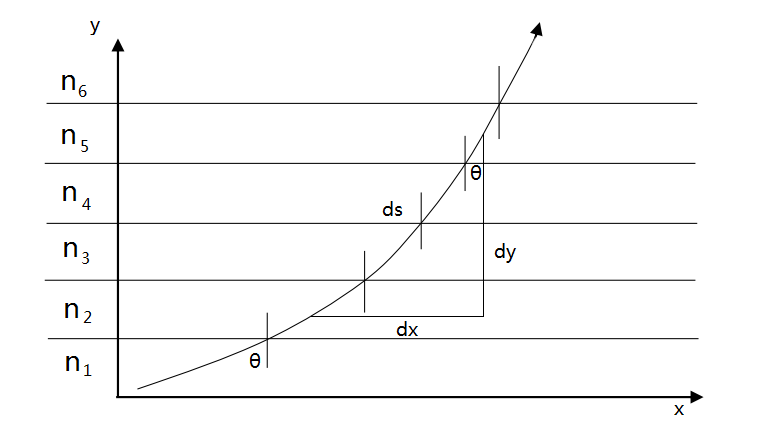
\includegraphics[width=0.5\linewidth]{guangxianchuanbo.PNG}
\caption{在非均匀连续分层介质中的光线传输}
\label{fig:guangxianchuanshu}
\end{figure}

当折射率连续变化,光线传输路径将变成一条连续的曲线,令$ds$表示表示光传输路径上的一小段弧长,则$(\mathrm{d}s)^2=(\mathrm{d}y)^2+(\mathrm{d}x)^2$,从图\ref{fig:guangxianchuanshu}可以看出$\mathrm{d}x/\mathrm{d}s=\sin\theta$,整合化简后,可以得到公式\eqref{eq:feijunyungl}。
\begin{equation}
\big(\frac{\mathrm{d}y}{\mathrm{d}z}\big)^2=\frac{n^2(y)}{n_1^2\sin^2\theta_1}-1
\label{eq:feijunyungl}
\end{equation}

该公式描述了在折射率分布确定情况下纵坐标随传输距离的变化,也就给出了光线的传播路径,如果对$x$微分,就能将光线传播方程化简,给出偏微分方程。
\begin{equation}
\frac{\mathrm{
d}^2y}{\mathrm{d}x^2}=\frac{1}{2n_1^2\sin^2\theta_1}\cdot\frac{\mathrm{d}n^2(y)}{\mathrm{d}y}
\label{eq:feijunyunglp}
\end{equation}

公式\eqref{eq:feijunyunglp}可以证明在均匀介质中,折射率$n(y)$是常数,等式右边为0,即$\mathrm{d}y/\mathrm{d}x^2=0$,表示光路是传播距离的一次函数,光线以直线传播,而在非均匀介质中,折射率的梯度变化导致光线以曲线形态传输,如果已知折射率分布及相应坐标,给出初始入射角,理论上就可以求解得到光传输路径,这就是光线传输的基本方程。

当考虑光线传输偏折,进一步分析光传输路径时,结合正弦折射定律,在介质折射率是连续且呈梯度变化的情况下,光线传输时会向着折射率较高的区域偏折,并且偏折角度大小应该与光路长度和折射率的梯度大小,同时如果折射率在平行于光传输方向有梯度变化时,并不会改变光走向,仅仅会改变光程大小。

由于光程可以说是光线在介质中所有可能路径的最小值,因此如果我们对公式\eqref{eq:guangcheng}应用费马原理,即光程的偏导数为零,这是一个变积分,可以用欧拉-拉格朗日方程表示,并且如果将光束入射方向定为x方向,进行消元化简后,可以得到如下方程组:
\begin{equation}
\left\{
\begin{aligned}
\frac{{\rm d}^2y}{{\rm d}x^2}=\Big[1+\Big(\frac{{\rm d} y}{{\rm d}x}\Big)^2+\Big(\frac{{\rm d}z}{{\rm d}x}\Big)^2\Big]\cdot
\Big[\frac{1}{n}\Big(\frac{\partial n}{\partial y}-\frac{{\rm d}y}{{\rm d}x}\cdot\frac{\partial n}{\partial x}\Big)\Big]\\
\frac{{\rm d}^2z}{{\rm d}x^2}=\Big[1+\Big(\frac{{\rm d} y}{{\rm d}x}\Big)^2+\Big(\frac{{\rm d}z}{{\rm d}x}\Big)^2\Big]\cdot
\Big[\frac{1}{n}\Big(\frac{\partial n}{\partial z}-\frac{{\rm d}z}{{\rm d}x}\cdot\frac{\partial n}{\partial x}\Big)\Big]
\end{aligned}\right.
\label{eq:feijunyunchuanshu}
\end{equation}
式中,$\dfrac{{\rm d}y}{{\rm d}x},\dfrac{{\rm d}z}{{\rm d}x}$表示入射光线的斜率,如果光束入射方向与坐标轴x平行,则有$\dfrac{{\rm d}y}{{\rm d}x}=\dfrac{{\rm d}z}{{\rm d}x}=0$,其他情况下入射光的斜率应均不等于零。对方程组\eqref{eq:feijunyunchuanshu}进行积分就可以得到光线在非均匀介质中的传输路径,但是这种非线性问题比较难以求解,在具体结合流场求解时,可以根据网格来离散化求解。
\subsection{光程差及偏折角理论}
介质折射率与光线在介质中的几何路径的乘积就是光线的光程(Optical Path Length),如果假定光束沿着z方向传输,折射率经过介质的传输路径为$\text{OPL}(x,y,z,t)$,由定义可以知道光线传输的光程公式为式\eqref{eq:opl}。
\begin{equation}
\text{OPL}(x,y,t)=\int_{0}^{L}n(x,y,z,t)\text{d}z
\label{eq:opl}
\end{equation}
式中,由于考虑湍流的随机运动,引入了流场随时间变化,$n(x,y,z,t)$为流场在$t$时刻$(x,y,z)$处的折射率值。由于光速非常快,光线经过流场的时间很短,流场一般来不及发生变化,因此可以考虑流场冻结的方法,认为流场结构在光线经过时不发生改变。

在折射率不同的介质中传输时,光波传输的速度不同,由于频率不发生变化,波长也就不同,令真空中光速为$c$,波长为$\lambda$,介质中光速为$u$,波长为$\lambda_i$,则介质折射率可以由速度或者波长比值来表示,$n=c/u=\lambda/\lambda_i$。如果光线的传输路径为$s$,则波长数为$s\lambda_i$,可以推导出,在介质中的波长数与光程上的绝对波长数相同,即:$s/\lambda_i=s\cdot n/\lambda$。则光线传输路程上的相位变化为:$\phi=(2\pi/\lambda)\cdot\text{OPL}$。那么两条初始相位差为$\phi_0$的光线经过流场后的相位差则为:$\Delta\phi=(2\pi/\lambda)\cdot(\text{OPL}_1-\text{OPL}_2)+\phi_0$。

为了方便讨论,并且考虑到波面计算等问题,我们可以引入光程差(Optical Path Difference)的概念,即两束光在介质中经过一定传输距离后的光程之差,我们在本文定义流场中的光程差为折射率起伏与相应传输距离的乘积,如公式\eqref{eq:opd},在气动光学中,光线传输距离可以近似为流场厚度,因此折射率的起伏决定了光程差的大小。
\begin{equation}
\text{OPD}(x,y)=\int_{0}^{L}\Delta n(x,y,z)\text{d}z
\label{eq:opd}
\end{equation}
式中,$\Delta n(x,y,z)$为流场当前位置的折射率与流场平均折射率之差。

前文讨论到光线在不均匀介质中的传输路径应该为曲线,那么,当光线出射时,会有一个偏折角$\theta$,如果将光线的传输路径定义为$s$,根据正弦折射定律可以知道,偏折角的变化与折射率的梯度相同如公式\eqref{eq:opljiao}。
\begin{equation}
\text{d}\theta/\text{d}s=\nabla n
\label{eq:opljiao}
\end{equation}

光束沿z方向传播,偏折角在$x,y$方向上有$\theta_x,\theta_y$两个分量,由于本文考虑的产生气动光学效应的流场厚度较小,可以将传播路程$s$近似等于传播方向上的$z$坐标改变,可以得到偏折角计算公式\eqref{eq:pianzhejiao}。
\begin{equation}
\frac{\partial\theta_x}{\partial z}=\frac{\partial n}{\partial x}~;
~~~~\frac{\partial\theta_y}{\partial z}=\frac{\partial n}{\partial y}
\label{eq:pianzhejiao}
\end{equation}
式中,偏折角分量及总偏折角应满足$\theta_x^2+\theta_y^2=\theta^2$关系。

通过光束传播过程中产生的偏折角,我们可以计算由此导致的瞄准误差$\beta_{BSE}$,瞄准误差实际上可以作为像偏移的简单判断,它可以用采样时间过程中的偏折角平均值表示:
\begin{equation}
\beta_{BSE}=\frac{1}{M}\sum\limits_{i-1}^{M}\theta_i
\end{equation}
式中,$\theta_i$表示第$i$个时间步长产生的偏折角,$N$是采样样本个数。
\section{流场引起的光学畸变分析}
光束在经过非均匀流场时会产生像差,根据光束在传播过程中的波动性比较明显的结论,可以通过衍射角度来分析流场引起的光学畸变现象,同时可以进一步分析出流场折射率随机脉动起伏对光学成像的影响,最后应该考虑如何评价这些气动光学效应。
\subsection{基于衍射理论的像差分析}
光在传输过程中的波动性较为明显,尤其是光在通过尺寸较小的小孔传播时,可以用衍射方法来分析传播过程,衍射问题也是光学中最困难的问题之一,难以得到解析解,在求解过程中,通常需要对其进行近似处理。

通过对\eqref{eq:guangbodong}的求解,假设在真空中考虑,令孔径面积为$A_0$,波长为$\lambda$,$U(x_0,y_0,0)$为初平面上光场分布,距离初平面$Z$的接受面光场分布为$U(x,y,Z)$,则有式\eqref{eq:guangbodongjie}。
\begin{equation}
U(x,y,Z)=-\frac{i}{\lambda}\int\frac{U_0(x_0,y_0,0)\cdot e^{ikr}}{r}\cdot\text{d}A_0
\label{eq:guangbodongjie}
\end{equation}
式中,$r=Z-xx_0/Z-yy_0/Z$。

在光波传输过程中,可以利用频谱分析方法把光波的振幅随空间位置的变化关系转换到随空间频率的变换,例如在垂直$z$轴的截平面上,平面波振幅$U(x,y)$可以通过空间频率$(\nu_x,\nu_y)$表示,如公式\eqref{eq:fuliye}。
\begin{equation}
U(x,y)=\iint_{-\infty}^{+\infty}A(\nu_x,\nu_y)\cdot\text{exp}[i2\pi(\nu_xx+\nu_yy)]\text{d}\nu_x\text{d}\nu_y
\label{eq:fuliye}
\end{equation}
式中,$\text{exp}[i2\pi(\nu_xx+\nu_yy)]$称为相位因子。这种表示方法将空间任意点的振幅$U(x,y)$利用空间频率表示,$A(\nu_x,\nu_y)$表示任意一个频率$(\nu_x,\nu_y)$所占的比例,该公式把一个平面的光波分解为沿着空间不同方向传播的平面波,每个平面波对应着一组空间频率$(\nu_x,\nu_y)$,这个频域函数$A(\nu_x,\nu_y)$就叫做角谱。

利用角谱可以在频率层面表示光传输过程,而通过对\eqref{eq:fuliye}进行傅里叶逆变换可以得到角谱$A(\nu_x,\nu_y,z)$的传播公式,也就确立了光波传输过程,将角谱公式代入波动方程后,经过变换积分计算化简后,得到公式\eqref{eq:kongjingjiaopu}。
\begin{equation}
A(\nu_x,\nu_y,z)=A_0(\nu_x,\nu_y)\cdot\exp(ikz)\cdot\exp\big[-i\pi\lambda z(\nu_x^2+\nu_y^2)\big]
\label{eq:kongjingjiaopu}
\end{equation}
式中,令$H(\nu_x,\nu_y)=\exp(ikz)\cdot\exp\big[-i\pi\lambda z(\nu_x^2+\nu_y^2)\big]$就是在折射率为1的自由空间中的传递函数,只要求出初平面的角谱分布,再与传递函数$H(\nu_x,\nu_y)$相乘,通过傅里叶逆变换就可以得知在$z=$z平面处的振幅分布。

在直角坐标系中,光沿z轴方向传播,假设在初平面上光波表示为$U(x,y,0)$,经过传输距离$z$后,到达z$=z$平面的光波为$U(x,y,z)$,通过傅里叶变换就可以得到平面波的角谱衍射理论基本公式\eqref{eq:jiaopuyanshe}。
\begin{equation}
\begin{aligned}
U(x,y,z)=&\int\limits_{-\infty}^{+\infty}\!\int\limits_{-\infty}^{+\infty}U(x,y,0)\cdot\exp\big[\frac{i2\pi z}{\lambda}(1-\lambda^2\nu_x^2-\lambda^2\nu_y^2)^{1/2}\big]\cdot\\
&\exp\Big\{i2\pi\big[\nu_x(x-x_0)+\nu_y(y-y_0)\big]\Big\}\text{d}\nu_x\text{d}\nu_y\text{d}x_0\text{d}y_0
\end{aligned}
\label{eq:jiaopuyanshe}
\end{equation}

在紧靠着孔径的地方光场分布一般遵循几何光学的规律,与光学孔径形状类似,但随着传输距离的增加,光场会发生衍射,光斑将会扩散,光强分布发生了明显改变,我们把从产生衍射的区域到无穷远处称为菲涅尔衍射区域,如果传输距离较远,衍射图像扩散严重,光强减弱较多,我们把这个区域称为夫琅禾费衍射区或者远场衍射,相对应的较近的地方称为近场衍射,可以看出菲涅耳衍射区包含了夫琅禾费衍射区。

为了能够通过计算得到衍射图像,通常都需要进行适当的近似,若考虑观测衍射成像的平面距离小孔$z$远大于孔径尺度,并且观测z轴附近的衍射情况,可以对一些参数进行近似处理,可见公式\eqref{eq:feijinsi}。
\begin{equation}
(1-\lambda^2\nu_x^2-\lambda^2\nu_y^2)^{1/2}\approx1-\frac{\lambda^2}{2}(\nu_x^2+\nu_y^2)
\label{eq:feijinsi}
\end{equation}

利用公式\eqref{eq:feijinsi}化简公式\eqref{eq:jiaopuyanshe},由于初平面孔径外的光场为零,因此可以只对孔径内部平面进行积分,先完成$\nu_x,\nu_y$的积分,利用傅里叶变换关系后可以得到菲涅尔衍射公式\eqref{eq:feinieer}。
\begin{equation}
\begin{aligned}
U(x,y,z)=&\frac{\exp(ikz)}{i\lambda z}\cdot\exp\big[\frac{ik}{2z}(x^2+y^2)\big]\int\limits_{-\infty}^{+\infty}\int\limits_{-\infty}^{+\infty}U(x_0,y_0,0)\cdot\\
&\exp\big[\frac{ik}{2z}(x_0^2+y_0^2)\big]\cdot\exp\Big[\frac{-i2\pi}{\lambda z}(xx_0+yy_0)\Big]\text{d}x_0\text{d}y_0
\end{aligned}
\label{eq:feinieer}
\end{equation}

由于式\eqref{eq:feinieer}中的相位因子$\exp\big[\frac{ik}{2z}(x_0^2+y_0^2)\big]$加大了计算积分的难度,在此如果令$z\gg\dfrac{k}{2}(x_0^2+y_0^2)$,可以把二次的相位因子在孔径上的积分近似为1,这种对于传输距离的较远的近似称作夫琅禾费近似,化简后可以得到夫琅禾费衍射公式\eqref{eq:fulanghefei},可以观察到光场分布就是小孔孔径上光场的傅里叶变换。
\begin{equation}
\begin{aligned}
U(x,y,z)=&\frac{\exp(ikz)}{i\lambda z}\cdot\exp\big[\frac{ik}{2z}(x^2+y^2)\big]\int\limits_{-\infty}^{+\infty}\int\limits_{-\infty}^{+\infty}U(x_0,y_0,0)\cdot\\
&\exp\Big[\frac{-i2\pi}{\lambda z}(xx_0+yy_0)\Big]\text{d}x_0\text{d}y_0
\end{aligned}
\label{eq:fulanghefei}
\end{equation}

夫琅禾费的衍射积分公式对条件要求非常高,它要求传输距离$z$远远大于孔径尺寸,假设光波为单色波,波长$\lambda$为600nm,那么当孔径尺寸$\Omega=0.25$mm时,传输距离$z$应该大于1.6m,若孔径尺寸$\Omega=0.025$m,那么观察距离必须大于1.6km才行,因此需要在远处才能观察到夫琅禾费衍射现象。

在以上衍射公式计算过程中,忽略了折射率的随机变化,直接令折射率为1,没有引入流场的随机特性,而在实际操作中,需要考虑折射率脉动引起的相位变化,假设在初平面$z=0$上有一个初始相位$\phi(x_0,y_0)$,在从初平面到$z=Z$平面传播过程中,相位畸变$\phi(x_0,y_0)$会有一个叠加累计,见公式\eqref{eq:xiangweicha}。
\begin{equation}
\Delta\phi=\int_{0}^{Z}\Delta n(x_0,y_0,z)\text{d}z
\label{eq:xiangweicha}
\end{equation}
式中,$\Delta n(x_0,y_0,z)$是初平面一点到$z=Z$平面上对应点传输路径中的折射率脉动。

因此当光在折射率随机非均匀分布的介质中传输时,引入相位变化后,在传输距离为$z$处的菲涅尔衍射公式\eqref{eq:fresnel}及夫琅禾费衍射公式式\eqref{eq:fraunhofer},这种基于折射率分布的衍射公式可以用来分析非均匀介质中的光波传输特性。
\begin{numcases}{}
\begin{aligned}
U(x,y,z)=&\frac{\exp(ikz)}{i\lambda z}\int\limits_{-\infty}^{+\infty}\int\limits_{-\infty}^{+\infty}U(x_0,y_0,0)\cdot\exp(ik\Delta\phi)\cdot\\
&\exp\Big\{i\frac{k}{2z}\big[(x-x_0)^2+(y-y_0)^2\big]\Big\}\text{d}x_0\text{d}y_0
\label{eq:fresnel}
\end{aligned}
\\
\begin{aligned}
U(x,y,z)=&\frac{\exp(ikz)}{i\lambda z}\int\limits_{-\infty}^{+\infty}\int\limits_{-\infty}^{+\infty}U(x_0,y_0,0)\cdot\exp(ik\Delta\phi)\cdot\\
&\exp\Big[-i\frac{k}{z}(xx_0+yy_0)\Big]\text{d}x_0\text{d}y_0
\label{eq:fraunhofer}
\end{aligned}
\end{numcases}

上节提到偏折角也是一个光传输过程中的重要参量,显示了光线在非均匀介质中传输一段距离后与入射方向的偏离角度,当引入偏折角概念时,由于传输距离Z相对于孔径尺寸非常大,可以近似地令$\theta_{x}=x/\text{Z},\theta_{y}=y/\text{Z}$,同时波数$k$表示为$2\pi/\lambda$,可以得到存在相位变化时,远场衍射的光波强度分布,同时在平面上观测时,可以消去$\exp(ikz)$这一项,得到远场光强分布公式\eqref{eq:yanshejiao}。
\begin{equation}
\begin{aligned}
U(\theta_{x},\theta_{y})=&\frac{-i}{\lambda \text{Z}}\iint\limits_\Sigma U(x,y,0)\cdot\exp\Big[ik\int_{0}^{\text{Z}}\Delta n(x,y,z)\text{d}z\Big]\cdot\\
&\exp\big[-ik(x\theta_{x}+y\theta_{y})\big]\text{d}x\text{d}y
\end{aligned}
\label{eq:yanshejiao}
\end{equation}
式中,$\Sigma$表示小孔区域,由于在孔径外光强都为0,因此仅对孔径内区域积分。

在非均匀介质中,光束的强度在传输过程中会有一定减弱,我们可以通过上述的衍射公式得到衍射的光场,然后利用该分布计算出成像平面的光强分布,假设远场的偏折角分量为$(\theta_x,\theta_y)$,在像平面$z=Z$处的衍射光强分布\cite{qiong2013}可以由公式\eqref{eq:yansheqiangdu}得到。
\begin{equation}
\begin{aligned}
I(\theta_x,\theta_y)=&U\cdot U^*=\frac{1}{\lambda^2Z^2}\iiiint U(x,y)\cdot U(x',y')\cdot\\
&\exp\Big\{ik\Big[\int\Delta n(x,y,z)\text{d}z-\Delta n(x',y',z')\text{d}z'\Big]\Big\}\cdot\\
&\exp\big[-ik\theta_x(x'-x)\big]\exp\big[ik\theta_y(y'-y)\big]\text{d}x'\text{d}y'\text{d}x\text{d}y
\end{aligned}
\label{eq:yansheqiangdu}
\end{equation}
式中,$\exp\big\{ik\big[\int\Delta n(x,y,z)\text{d}z-\Delta n(x',y',z')\text{d}z'\big]\big\}$体现了随机介质对光强度的影响,可以利用折射率脉动随时间的高斯分布将其变形,如公式\eqref{eq:gaosifenbu}。
\begin{equation}
\exp\Big\{-\frac{1}{2}k^2<\Big[\int\Delta n(x,y,z)\text{d}z-\Delta n(x',y',z')\text{d}z'\Big]^2>\Big\}
\label{eq:gaosifenbu}
\end{equation}

令流场的积分尺度大小为$\Lambda$,通过坐标系变换,能够得到爱里衍射斑的散射损失系数$\alpha$,爱里斑的强度分布可以通过公式\eqref{eq:yansheqiangdu}得到。
\begin{equation}
\begin{cases}
I(\theta)=\dfrac{I_0D^2}{4R^2\theta^2}\cdot J_I^2\big(\dfrac{\pi D\theta}{\lambda}\big)\\
\alpha=2k^2<\Delta n^2>\cdot\Lambda
\end{cases}
\end{equation}
式中,$I_0$为初平面的光波强度,$D$为小孔直径,$\lambda$为单色波波长,$J_I$为I阶的Bessel函数。第I阶贝塞尔函数$J_I(x)$可以表示为式\eqref{eq:ibessel}。
\begin{equation}
J_I(x)=\sum\limits_{m=0}^{\infty}\frac{(-1)^m}{m!\Gamma(I+m+1)}\Big(\frac{x}{2}\Big)^{I+2m}~~~~~~I\geq0
\label{eq:ibessel}
\end{equation}
式中,当I为整数时,有$(n+m)!=\Gamma(I+m+1)$,代入式\eqref{eq:ibessel},可以得到整数阶的贝塞尔函数。
\begin{equation}
J_I(x)=\sum\limits_{m=0}^{\infty}\frac{(-1)^m}{m!(I+m)!}\Big(\frac{x}{2}\Big)^{I+2m}~~~~~~I=0,1,2,\ldots
\label{eq:nbessel}
\end{equation}

由此,可以知道经过衍射后爱里斑的强度相对于初始强度的比值就可以通过损失系数$\alpha$确定,如公式\eqref{eq:jianruoyinzi}。
\begin{equation}
<\frac{I}{I_0}>=\exp\Big[-2k^2\int<\Delta n^2>\cdot\Lambda\text{d}z\Big]
\label{eq:jianruoyinzi}
\end{equation}

通过强度的比值公式可以看出,光在随机非均匀介质中传输时的光束强度变化与折射率的变化有直接关系,只要知道流场每一点的折射率分布,就能了解光束传输过程中的能量改变。
\subsection{气动光学的评价方法与评价指标}
光波经过随机非均匀流场会产生的波像差,这时在衍射像中的最大强度一定比同等情况下没有像差的系统中爱里斑中心强度小,这种情况导致了能量分布的变化,瑞利在研究这个现象的过程中发现,在观测截面查看有像差光学系统对光强分布影响时,如果波阵面偏离高斯参考球面的距离小于$1/4$波长,中心能量损失小于$20\%$,这种情况下系统对光学成像质量的影响不大,在可接受范围内,这也成为评价光学系统的一个重要指标,称为瑞利判据。

事实上,在分析光波经过流场后发生的波面畸变时,可以将光瞳函数$f(x,y)$分解为振幅$A(x,y)$和相位$\phi(x,y)$表示,如公式\eqref{eq:guangtonghanshu}。
\begin{equation}
f(x,y)=A(x,y)\cdot e^{-i\phi(x,y)}
\label{eq:guangtonghanshu}
\end{equation}
式中,光束截面的振幅一般起伏不大,对光瞳函数影响不大,可以令$A(x,y)\equiv1$,而波面的相位$\phi$是研究波面畸变的重点。

若令离参考面为传输距离的球面上相位变化平均为$\overline{\phi(x,y)}$,每一个波面点(x,y)上,光的波面畸变表示为$\Delta\phi(x,y)$,则有$\Delta\phi(x,y)=\overline{\phi(x,y)}-\phi(x,y)$。通过相位差就可以计算波面均方差$\sigma_\phi^2$,从而描述波面畸变情况\cite{haris2004},考虑到波动参数可能会随着时间变化,可以取系统平均,去除时间的影响,得到均方差公式\eqref{eq:junfangcha}。
\begin{equation}
\begin{aligned}
\sigma_\phi^2&=<\overline{[\overline{\phi(x,y)}-\phi(x,y)]^2}>
=<\overline{\phi^2(x,y)}>-<\overline{\phi(x,y)}>^2\\
&=\sigma_0^2-(\bar{\sigma}^2+\overline{K^2})
\end{aligned}
\label{eq:junfangcha}
\end{equation}
式中,$\sigma_0^2=<\overline{\phi^2(x,y)}>,\bar{\sigma}^2=<\bar{\phi}^2>,\overline{K^2}=<K^2(x^2+y^2)>$,$x,y$相互独立,$K$为倾斜因子,也可以沿角度方向测量相位变化,即$\overline{\phi(x,y)}=\bar{\phi}+K(x\cos\theta+y\sin\theta)$。波面均方差是用来计算气动光学效应的重要参数,尤其是涉及到斯特列尔比及光学传递函数的计算。

如果初平面的光场分布函数为$U(x,y)$,在观测平面及像平面的光场分布为$U(x',y')$,光瞳函数为$f(\eta,\xi)$,传输距离为Z,那么根据惠更斯-菲涅尔原理,可以得到$U(x',y')$表达式\eqref{eq:guangchang}。
\begin{equation}
\begin{aligned}
U(x',y')=&\text{C}\cdot\iint\limits_\Sigma U(x,y)\cdot\exp\Big[-i\frac{k}{\text{Z}}(x\eta+y\xi)\Big]\text{d}x\text{d}y\times\\
&\iint\limits_\Sigma f(\eta,\xi)\cdot\exp\Big[-i\frac{k}{\text{Z}}(x'\eta'+y'\xi')\Big]\text{d}\eta\text{d}\xi
\end{aligned}
\label{eq:guangchang}
\end{equation}
式中,$\Sigma$为孔径区域,若初平面的光源为点,则第一项积分为1,可以看出,光波在像面的振幅类似于是通过瞳函数经过傅里叶变换得到的,进行合适的坐标变换后,选择合适的归一化系数C,可以得到点振幅扩散函数$ASF(x',y')$,如公式\eqref{eq:dianzhenfu}。
\begin{equation}
ASF(x',y')=\text{C}\cdot\iint\limits_\Sigma f(x,y)\exp\Big[-i\frac{k}{Z}(xx'+yy')\Big]\text{d}z\text{d}y
\label{eq:dianzhenfu}
\end{equation}

通过点振幅扩散函数可以得到点扩散函数$PSF(x',y')$,它描述了光强度在像平面的相对分布,光场的强度正比于振幅的平方,可以得到点扩散函数$PSF(x',y')$。
\begin{equation}
PSF(x',y')=ASF(x',y')\cdot ASF^*(x',y')
\label{eq:diankuosan}
\end{equation}
式中,$ASF^*$表示点振幅扩散函数$ASF$的共轭。同时点扩散函数描述的是光强的相对分布,应满足$\iint\limits_{-\infty}^{+\infty}PSF(x',y')=1$,点扩散函数也可以作为一个描述流场气动光学效应的参量。

事实上只要对点扩散函数进行傅里叶变换,就可以得到流场的光学传递函数$OTF(f_{x'},f_{y'})$,也就能够从空间频率角度描述光传输效应
,如公式\eqref{eq:guangxuechuandi}。
\begin{equation}
OTF(f_{x'},f_{y'})=\iint PSF(x',y')\cdot\exp\big[-i2\pi(f_{x'}x'+f_{y'}y')\big]\text{d}x'\text{d}y'
\label{eq:guangxuechuandi}
\end{equation}

可以看出点振幅扩散函数、点扩散函数以及光学传递函数通过光瞳函数联系在一起,只要求出光瞳函数,或者说求出光波经过流场的相位畸变情况,就能够描述光束的传播过程,了解流场产生的气动光学效应,并且对其进行校正。

能够用来描述气动光学效应,对流场进行评估的另一个指标是斯特列尔比(strehl),它表示为有像差的衍射光斑的最大亮度$I$与同等传输距离下没有像差的衍射光斑的最大亮度$I_0$的比值\cite{mark2013},若传输距离为Z,可以由公式\eqref{eq:strehl}表示。由于一般光斑中心亮度最大,因此又将其称为中心亮度判据,可以作为判断图像能否分辨的依据。
\begin{equation}
S_\text{Z}=I/I_0
\label{eq:strehl}
\end{equation}

斯特列尔比可以通过点波面误差、点扩散函数、光学传递函数、泽尼克圆多项式等多种方法计算,由于定义简单并且比较容易计算,这是一种目前比较常用的评估气动光学效应的方法。本文定义的像点光强$I$为这一点光场分布的模的平方,并且需要对时间取平均,在极坐标下,可以利用点扩散函数得到像点光强$I(Q_\phi)$。
\begin{equation}
I(Q_\phi)=\Big(\frac{Aa^2}{\lambda Z^2}\Big)^2\cdot\bigg\vert\int_0^1\int_0^{2\pi}\exp\Big\{i\big[k\phi-\nu\rho\cos(\theta-\psi)-\frac{1}{2}u\rho^2\big]\Big\}\rho\text{d}\rho\text{d}\theta\bigg\vert^2
\end{equation}
式中,令$u,\nu$为0,就能得到无像差时像点的最大光强$I(Q_0)$。因此斯特列尔比可以表示为公式\eqref{eq:strehldiankuosan}。
\begin{equation}
S_\text{Z}(Q)=\frac{I(Q_\phi)}{I(Q_0)}=\frac{1}{\pi^2}\cdot\bigg\vert\int_0^1\int_0^{2\pi}\exp\Big\{i\big[k\phi-\nu\rho\cos(\theta-\psi)-\frac{1}{2}u\rho^2\big]\Big\}\rho\text{d}\rho\text{d}\theta\bigg\vert^2
\label{eq:strehldiankuosan}
\end{equation}

根据统计光学原理,可以通过光学传递函数来表示中心光强的比值,通常情况下由于光学传函数在积分宽度上并不是均匀变化的,因此可以利用系统平均处理,假设系统总的光学传递函数为$f_0(x,y)$,通过波面均方差$\sigma_\phi^2$,结合光学传递函数,可以得到中心光强的比值,见公式\eqref{eq:strehlchuandi}。
\begin{equation}
\begin{aligned}
<I/I_0>&=\frac{4}{\pi}\iint\limits_{-\infty}^{+\infty}\exp(-k^2\sigma_\phi^2[1-r(x,y)])\cdot f_0(x,y)\text{d}x\text{d}y\\
&=\frac{4}{\pi}\exp(-k^2\sigma_\phi^2)\iint\limits_{-\infty}^{+\infty}\exp\big[k^2\sigma_\phi^2r(x,y)\big]\cdot f_0(x,y)\text{d}x\text{d}y
\end{aligned}
\label{eq:strehlchuandi}
\end{equation}
式中,$r(x,y)$为相位差$\Delta\phi$的相关系数。将指数部分用泰勒级数展开:
\begin{equation}
\exp\big[k^2\sigma_\phi^2r(x,y)\big]=\sum\limits_{n=0}^{\infty}\frac{(k^2\sigma_\phi^2)^n}{n!}\cdot r^n(x,y)
\end{equation}
上式代入\eqref{eq:strehlchuandi}后,对其进行近似处理,令孔径尺寸D远大于折射率脉动尺寸$l_x,l_y$,再通过级数展开,可以得到大孔径近似下的斯特列尔比,如公式\eqref{eq:streldakongjing}。
\begin{equation}
\begin{cases}
<I/I_0>\sim\exp(-k^2\sigma_\phi^2)\Big\{1+\dfrac{8\cdot F(k^2\sigma_\phi^2)}{(\text{D}/l_x)(\text{D}/l_y)}\Big\}\\
F(x)=\sum\limits_{n=1}^{\infty}\dfrac{x^n}{n^2\cdot n!}~~~~~~~~~~~(x=k^2\sigma_\phi^2)
\end{cases}
\label{eq:streldakongjing}
\end{equation}

可以将式\eqref{eq:streldakongjing}的光强比值分为两部分,第一部分为$\exp(-k^2\sigma_\phi^2)$影响衍射极限,削弱光强,第二部分则对分布更广更分散的光束产生影响,Hogge认为这种光束属于非相干光束,如果衍射孔径足够大,满足D>$6l_x$,就可以忽略第二项的影响。

公式\eqref{eq:junfangcha}给出了波阵面的相位均方差$\sigma_\phi^2$,在通过波面误差来计算斯特列尔比时,我们假设波像差的均方值在像差不大的情况下能够表示参考球面中心的光强,此时斯特列尔比能表示为公式\eqref{eq:strehljunfangcha}。
\begin{equation}
S_\text{Z}(Q)=e^{-k^2\cdot\sigma_\phi^2}
\label{eq:strehljunfangcha}
\end{equation}

对比公式\eqref{eq:streldakongjing}、\eqref{eq:strehljunfangcha},可以发现当作大孔径近似处理即令D$>6l_x$时,利用光学传递函数得到的斯特列尔比与直接利用波面相位均方差得到的结果一致。至此,可以发现只要能够给传输路径中空间每点的出折射率分布,就能利用点扩散函数来描述成像的模糊情况,用斯特列尔比来描述光强度的衰减,还可以利用偏折角来体现光学成像的偏移,利用光学传递函数(OTF)就可以得到像面光场分布,从而对气动光学效应进行评价,为进一步的光学校正提供基础。
\section{高速流场中的气动光学计算分析}
在飞行器高速飞行时,周围空气与其相互作用,会形成复杂的湍流流场,对于流场的光学特性研究,可以将其分为平均流场及随机脉动流场两种情况分别分析,平均流场主要依据光线追迹理论,对光程差、传输方程等进行计算,而湍流部分主要依据统计学理论进行分析。一般对光束经过流场前后的畸变进行分析时,可以计算通过流场作用后的光波再经过光学透镜成像,从而对其进行气动光学效应的具体分析,其成像机理如图\ref{fig:qidongguangxuejisuanjili}。

\begin{figure}[bhtp]
\centering
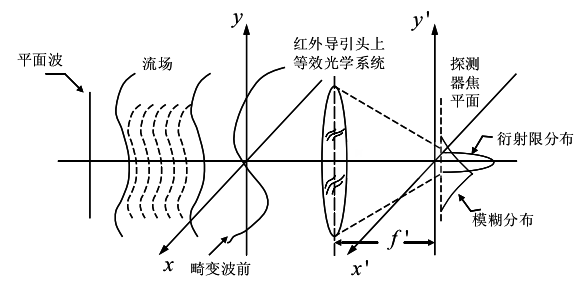
\includegraphics[width=0.8\linewidth]{qidongguangxuejili.PNG}
\caption{光束经过流场后的计算分析图}
\label{fig:qidongguangxuejisuanjili}
\end{figure}
\subsection{平均流场的光传输计算}
飞行器外的流场随飞行过程不断变化,不具有空间、时间不变性,无法应用线性光学的理论描述,但是抛开流场随机脉动部分,考虑稳定的层流部分时,由于这部分的流场比较稳定,可以认为不随时间变化。层流流场的密度在空间上呈现不均匀分布,对其气动光学效应分析时,可以利用光线追迹法得到光在流场中的传输路径,从而了解光程差、相位差等参数。

在通过光线追迹法计算具体流场的光程差时,一般先通过计算流体力学的相关知识得到流场中的密度、温度、压强等物理参量,继而通过这些参数来计算流场的诸如波面畸变、点扩散函数等气动光学效应。由于对流场的模拟一般会将三维区域划分成多个小单元构成的网格结构,因此在计算光程差时,可以通过计算每个小单元中的光程差然后累加得到,如公式\eqref{eq:lisanguagnchengcha}。
\begin{equation}
L_{OPD}=\sum\limits_{i=1}^{N}\Delta n_i\cdot\Delta l_i
\label{eq:lisanguagnchengcha}
\end{equation}
式中,$\Delta n_i$为第$i$个单元中心的折射率与平均流场的折射率之差,$\Delta l_i$为光线经过第$i$个单元上下表面的实际路程。

这样通过网格单元离散单元的光程差进行叠加后就可以得到光束穿过整个流场区域的光程差,如果定义光波波数$k=2\pi/\lambda$,将波数与光程差相乘就能够得到光束的相位差,也就能够分析光束波面畸变情况。

平均流场对光束传输产生的像偏移可以通过偏折角来快速、直观地表示,通过\eqref{eq:pianzhejiao},结合光程差概念,假设光束沿z方向进入流场,那么就可以计算出光束在像面沿$x,y$方向的偏折角$\theta_x,\theta_y$,如公式\eqref{eq:pingjunpianzhejiao}。
\begin{equation}
\left\{
\begin{aligned}
\theta_x&=\frac{\partial L_{OPD}}{\partial x}=\frac{\partial}{\partial x}\int_0^L\Delta n(x,y,z){\rm d}z\\
\theta_y&=\frac{\partial L_{OPD}}{\partial y}=\frac{\partial}{\partial y}\int_0^L\Delta n(x,y,z){\rm d}z
\end{aligned}
\right.\label{eq:pingjunpianzhejiao}
\end{equation}

通过偏移角来衡量光斑相对中心的偏移主要基于流场折射率的起伏来得到,而折射率主要通过流场来影响,因此需要经过大量计算才能得到精确结果,而事实上当我们需要快速直观地对飞行器周围流场进行大致像偏移的评估时,可以根据一些流场已知参数直接判断。如果我们知道了来流速度或者飞行器飞行速度$u$,给出飞行器头部的半锥角$\alpha$,可以通过式\eqref{eq:jibojiao}知道头部激波角$\theta$。
\begin{equation}
\tan\alpha=\frac{(u\sin\theta)^2-1}{\Big(\dfrac{\gamma+1}{2}u^2-\sin^2\theta+1\Big)\tan\theta}
\label{eq:jibojiao}
\end{equation}
式中,$\gamma$为流场气体的比热比。

令G-D系数为$K_{\rm GD}$,$\beta$为入射光线与飞行器中轴的夹角,$\rho_0,\rho_1$分别为远场密度以及激波后的密度,$\delta$为像偏移角,通过这些基本参数就可以得到大致像偏移情况。
\begin{equation}
\left\{
\begin{aligned}
\frac{\cos(\theta+\beta)}{\cos(\theta+\beta+\delta)}=\frac{1+K_{\rm GD}\cdot\rho_1}{1+K_{\rm GD}\cdot\rho_0}\\
\rho_1=\rho_0\cdot\frac{(\gamma+1)u^2\sin^2\theta}{(\gamma-1)u^2\sin^2\theta+2}
\end{aligned}
\right.\label{eq:jibopianyi}
\end{equation}

公式\eqref{eq:jibojiao}及\eqref{eq:jibopianyi}联立,就能够通过飞行器本身结构参数、流场速度、远场的密度以及入射光线的入射角度四个已知的物理参量计算得到像偏移情况,这种方法在计算简单、方便的同时牺牲了一些精确度,没有通过流场内部结构来分析光束的传输,一般情况下,这种近似计算可以用来大致地快速分析流场产生的像偏移,对此有一个宏观上的判断。

在通过光线追迹法结合计算流体软件网格划分离散计算得到光线经过每个小单元格的光程差,累加后能得到穿过流场后每一点的全部光程差,如果假设光束穿过流场时的光程差分布为$P(x,y)$,并且忽略瞄准误差,那么对其作傅里叶变换,就可以得到焦平面上的光场分布,令小孔直径为D,$\theta_x,\theta_y$为孔径投射到像平面的角坐标,我们可以得到像面上的光场分布及光强分布如式\eqref{eq:guangchangfenbu}、\eqref{eq:guangqiangfenbu}。
\begin{align}
U(\theta_x,\theta_y)&=\bigg(\frac{4}{\pi\text{D}^2}\bigg)\cdot\int_{-\frac{\text{D}}{2}}^{\frac{\text{D}}{2}}\int_{-\sqrt{(\text{D}/2)^2-x^2}}^{\sqrt{(\text{D}/2)^2-x^2}} e^{-ikP(x,y)}\cdot e^{ik(\theta_x,\theta_y)}\text{d}x\text{d}y
\label{eq:guangchangfenbu}\\
I(\theta_x,\theta_y)&=\big|U(\theta_x,\theta_y)\big|^2
\label{eq:guangqiangfenbu}
\end{align}

因此如果能够计算出光学窗口处流场的光程差,就能得到时间上近似稳定的平均流场对光束传输的影响,可以通过定义光学孔径,同时忽略瞄准误差,采用二元的傅里叶变换的方法,就能计算出平面光经过流场后的光场分布情况。
\subsection{湍流流场的光传输计算}
在考虑湍流引起的光学传输特性变化时,由于湍流运动的随机性,可以通过统计特性来描述流场中空气的运动规律,通常情况下可以引入亚格子模型分析湍流折射率脉动,湍流的气动光学效应可以认为是沿着光传输方向的累加产生的。亚格子模型主要利用相关函数来描述密度脉动情况,一般可以采用冯$\cdot$卡门模型、高斯模型及指数模型三种,假设密度相关函数为$C(x,y,z)$。
\begin{align}
&\text{冯$\cdot$卡门模型:}
&C(x,y,z)&=\frac{2^{2/3}}{\Gamma(1/3)}(l_{xyz})^{1/6}\cdot B_{1/3}\big[(l_{xyz})^{1/2}\big]\\
&\text{高斯模型:}
&C(x,y,z)&=\exp[-l_{xyz}]\\
&\text{指数模型:}
&C(x,y,z)&=\exp\big[-(l_{xyz})^{1/2}\big]\label{eq:zhishuxiangguanxishu}
\end{align}
式中,$l_{xyz}=(x/l_x)^2+(y/l_y)^2+(z/l_z)^2$,$\Gamma(1/3)$是Gamma函数,$B_{1/3}\big[(l_{xyz})^{1/2}\big]$是第二类修正Bessel函数。

波面的畸变可以通过折射率协方差来计算,如果假设均方差折射率脉动为$\overline{n'^2}$,湍流密度相关系数定为$C(x,y,z)$,可以得到折射率协方差公式。
\begin{equation}
R(x,y)=\int_0^\text{L}\int_{-\text{Z}}^{\text{L}-\text{Z}}\overline{n'^2}(x',y',z')\cdot C(x,y,z)\text{d}z\text{d}z'
\label{eq:zheshelvxiefangcha}
\end{equation}

通过以上公式,可以完整地表示沿传输方向的折射率变化,得到相位的方差、相关函数及相关长度。
\begin{align}
&\text{相位方差:}&\sigma_\phi^2=k^2\cdot R(0,0)\label{eq:xiangweifangcha} \\
&\text{相位相关函数:}&C_\phi(x,y)=k^2\cdot\phi(x,y) \\
&\text{相位相关尺度:}&l_\phi=\frac{1}{\sigma^2}\int_{-\infty}^{\infty}\int_{-\infty}^{\infty}C_\phi(x,y)\text{d}x\text{d}y \label{eq:xiangweixiangguanchangdu}
\end{align}

可以发现,湍流密度相关系数影响了相位变化的计算,相位方差可以利用相位相关长度与折射率脉动的均方差联合表示,取加权函数为1后,得到公式\eqref{eq:xiangweijunfangcha}
\begin{equation}
\sigma_\phi^2=2k^2\int_0^\text{L}\overline{n'^2}(z)l_\phi\text{d}z
\label{eq:xiangweijunfangcha}
\end{equation}

对相位相关函数进行傅里叶变换就可以得到湍流相位脉动功率谱,取$x,y$方向上的空间频率分别为$\nu_x,\nu_y$,相位脉动功率谱可以表示为\eqref{eq:xiangweimaidong}
\begin{equation}
F_\phi(\nu_x,\nu_y)=\frac{1}{(2\pi)^2}\int_{-\infty}^{\infty}\int_{-\infty}^{\infty}C_\phi(x,y)\cdot\exp[-i(\nu_xx+\nu_yy)]\text{d}x\text{dy}
\label{eq:xiangweimaidong}
\end{equation}

通过功率谱函数$F_\phi(\nu_x,\nu_y)$可以求出湍流介质中时间平均的调制传递函数$f_{MTF}(\nu_x.\nu_y)$,从而用亚格子模型描述了湍流对光传输路径的影响。
\begin{align}
&f_{MTF}(\nu_x,\nu_y)=\exp\big\{-\big[C_{\phi B}(0,0)-C_{\phi B}(\nu_x,\nu_y)\big]\big\}\\
&C_{\phi B}(\nu_x,\nu_y)=\int_{-\infty}^{\infty}\int_{-\infty}^{\infty}F_\phi(\nu_x,\nu_y)\cdot\exp\big[-i(\nu_xx+\nu_yy)\big]\text{d}x\text{d}y
\end{align}
式中,$C_{\phi B}(\nu_x,\nu_y)$为相位相关函数,与功率谱$F_\phi(\nu_x,\nu_y)$有关。

对于包含湍流流场的混合流场的气动光学效应,就可以利用光经过平均流场在焦平面所成像的点扩散函数PSF与相对应的调制传递函数$f_{MTF}$通过卷积得到像的强度分布$I$。
\begin{equation}
I\Big(\frac{x}{\lambda f},\frac{y}{\lambda f}\Big)=\mathscr{F}^{-1}\big\{f_{MTF}(\nu_x,\nu_y)\big\}*\mathscr{F}\Big\{PSF\big(\frac{x}{\lambda f},\frac{y}{\lambda f}\big)\Big\}
\end{equation}
式中,$f$为光瞳到焦平面距离即焦距,$\mathscr{F}$为傅里叶变换。

对于时间平均流场能够采用光线追迹法计算出光束的偏折角,而对于湍流脉动流场,可以通过偏折角的均方差来描述湍流场对光束的影响。在利用统计方法计算得到折射率均方差的基础上,通过下式得到偏折角均方差。
\begin{equation}
\overline{\Delta\theta^2}=-\overline{\Delta n^2}\cdot H\int_0^\infty\frac{1}{r^2}\cdot\frac{\rm d}{{\rm d}r}\Big(\frac{r^2{\rm d}C_n(\Delta x,\Delta y,\Delta z)}{{\rm d}r}\Big){\rm d}r
\end{equation}
式中,$C_n(\Delta x,\Delta y,\Delta z)$是折射率相关函数,可以选择不同的经验模型进行计算,$r=\sqrt{\Delta x^2+\Delta y^2+\Delta z^2}$,H为传输距离,在湍流场中的近距离传输下可以近似为流场厚度。

至此,利用光程差、偏折角等可以描述出时间平均流场对光传输的影响,通过偏折角均方差可以表述湍流部分对光传输特性的影响,利用光学传递函数能够描述出光束经过混合流场的光强分布情况,基于这些气动光学效应的描述、计算方法,为应用中的光学校正以及气动光学效应的削弱方法提供有力的理论基础和前期准备。
\section{本章小结}
本章主要阐述了光波在非均匀介质中的传输、衍射理论,讨论了非均匀介质引起的波面畸变现象,将流场对光传输的影响划分为平均流场及随机脉动流场分别作用后效果的叠加,推导了波前畸变计算公式,对斯特列尔比、点扩散函数、光学传递函数等光学评价指标进行了推导计算,并且研究了高速流场中如何对流场的稳定部分及随机部分的气动光学效应进行计算,在平均流场部分采用光线追迹法求解出平均波面畸变,在随机脉动部分引入亚格子模型,主要通过功率谱函数及光学传递函数来计算像面光强分布,描述光束传播过程。%--第四章--
%\chapter{光传输特性的模拟及计算}
数值模拟是研究气动光学效应的有效手段,相对实验研究而言,采用数值模拟方法可以更加全面地控制模拟条件并且能够对模拟过程多次重复,给出正确的初始条件就可以得到精确且定量的结果,本章对于光学传输部分的数值计算均采用Mathematica数学计算工具。光场的重要参数~--~折射率能够通过流场密度转换得到,通过折射率的分布、起伏情况结合线性光学及统计光学等计算方法,就能描述出光束的传播过程。
\section{流场密度到折射率的转换及计算}
通过波动方程\eqref{eq:guangbodong}可以看出,光波的传输主要收到折射率分布的影响,由此可知研究光传输特性时,首先应该求流场的解折射率。气体的折射率往往受到流场的压力、密度及温度等状态参数影响,而一般情况下,气体的折射率大小主要取决于气体的密度,通过洛伦兹-洛伦茨公式,可以得到流场的密度与折射率之间的直接关系\cite{max2001},如式\eqref{eq:luolunzi}:
\begin{equation}
\Big(\frac{n^2-1}{n^2+2}\Big)\cdot\frac{1}{\rho}=\frac{2}{3}K_{GD}
\label{eq:luolunzi}
\end{equation}
式中,$K_{GD}$为气体密度到折射率的转换系数,称为$G-D$系数,$n$为气体折射率, $\rho$为气体密度,由于大气密度略大于1,可以进行简单的近似,即$n^2-1\approx2(n-1),n^2+1\approx3$,可以得到简单的密度到折射率的转换关系\cite{yxl2003qdgxyl}:
\begin{equation}
n=1+K_{GD}\cdot\rho
\label{eq:gdgongshi}
\end{equation}

标准空气的$G-D$系数与波长存在一定的函数关系,并且在红外区域,该系数基本保持不变,表达式可以近似为式:
\begin{equation}
K_{GD}=2.23\times 10^{-4}(1+\frac{7.52\times 10^{-3}}{\lambda^2})
\end{equation}
式中,$\lambda$为波长,单位$(\mu\text{m})$,$K_{GD}$单位$(\text{cm}^3/\text{g})$。本文计算并列举了$0.2\sim0.9\mu\text{m}$波长对应的$G-D$系数,如表\ref{tab:gdxishu}。
\begin{table}[bthp]
\caption{$G-D$系数表}
\label{tab:gdxishu}
\centering
\begin{tabular}{|c|c|c|c|}
\hline
波长($\mu \text{m}$)&$G-D$系数$(\text{cm}^3/\text{g})$&波长($\mu \text{m}$)&$G-D$系数$(\text{cm}^3/\text{g})$\\
\hline
0.2&0.2642&0.6&0.2220\\\hline
0.3&0.2385&0.7&0.2205\\\hline
0.4&0.2281&0.8&0.2201\\\hline
0.5&0.2236&0.9&0.2198\\\hline
\end{tabular}
\end{table}

通过折射率与密度的对应转换关系,就可以求出相应的折射率分布。本文以第三章中通过计算流体力学软件模拟得到的机载凸台周围流场为例,选取运行速度为2倍音速情况,为了比较清晰地展现高速流场的分布情况,可以以凸台光学窗口为基准截面,选取窗口周围约0.75m$\times$1.4m范围的长方形区域,利用公式\eqref{eq:gdgongshi}得到从密度到折射率的转换,如图\ref{fig:midudaozheshelv}。
\begin{figure}[bhtp]
\centering
\subcaptionbox{截面区域密度}{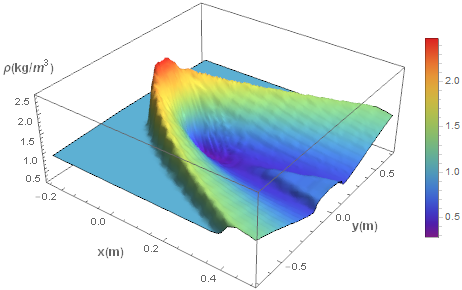
\includegraphics[width=0.49\linewidth]{tutaijiemianmidu.png}}
\subcaptionbox{截面区域折射率}{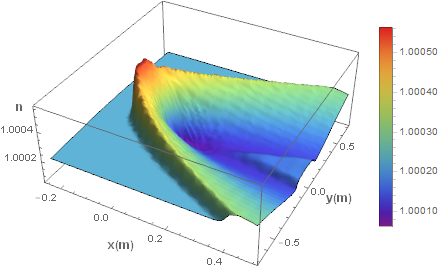
\includegraphics[width=0.49\linewidth]{tutaijiemianzheshelv.png}}
\caption{凸台周围截面密度及折射率分布情况}
\label{fig:midudaozheshelv}
\end{figure}

在图\ref{fig:midudaozheshelv}中,可以明确地看到剪切层的存在,并且剪切层中的密度及折射率比远处流场高,而在凸台正上方近壁面处,流场密度及折射率明显减弱,且低于平均值。根据第三章的分析,这是由于凸台顶部为半球,正中间处于最高位置,紧接着凸台结构呈下降趋势,这种结构的改变引起了高速流场的变化,在距离凸台底部高度为0.2m,以凸台中心为几何中心,尺寸为0.75m$\times$1.4m的长方形截面上,折射率波动位于1.00006$\sim$1.00056之间,正是这种不规则的折射率脉动起伏导致了光束传输过程中的畸变存在。
\section{光束的数学表达及衍射分析}
流场对光束的传输影响一般通过衍射理论来分析,利用流场密度转换成折射率后,通过折射率的脉动等参数计算出相位畸变、光学传递函数等,能够根据衍射图来评价流场对光传输的影响。
\subsection{基模高斯光束的传输特性}
通常情况下,光学设备接受、发射的激光光束均满足高斯分布,在所有可能的激光光束中基模高斯光束最具有典型性,它是一种具有特殊传输性质的高斯球面波,在研究中具有非常重要的作用,基模高斯光束的振幅表达式为\eqref{eq:gaosiguangshu}。
\begin{equation}
U(x,y,z)=\frac{A_0}{\omega(z)}\exp\big[\frac{-(x^2+y^2)}{\omega^2(z)}\big]\times\exp\big\{-ik\big[\frac{x^2+y^2}{2R(z)}+z\big]+i\varphi(z)\big\}
\label{eq:gaosiguangshu}
\end{equation}
式中,$z$为传输距离,$z$处光斑半径$\omega(z)=\omega_0\sqrt{1+(z/f)^2}=\omega_0\sqrt{1+[(\lambda z)/(\pi\omega_0^2)]^2}$,等相面曲率半径$R(z)=z[1+(f/z)^2]$,束腰半径$\omega_0=\sqrt{(\lambda f)/\pi}$,共焦参量$f=(\pi\omega_0^2)/\lambda$。

由式\eqref{eq:gaosiguangshu}可知,高斯光束的沿既定方向传播时会有一个特定的发散角,发散角与束腰半径成反比,而与波长成正比关系,束腰半径越小,它的光斑扩散越快。通过计算式,只要知道激光的波长,给定束腰半径,就可以知道在传输路径上每个截面上的光波表达式,从而知道光强分布。假设光斑的光强$I(x,y,z)$分布与振幅的模的平方相等,则可以令光强表示为\eqref{eq:guangqiang}。
\begin{equation}
\begin{aligned}
I(x,y,z)&=\big|U(x,y,z)\big|^2=U(x,y,z)\cdot U^*(x,y,z)\\
&=\frac{A_0^2}{\omega^2(z)}\exp\big[\frac{-2(x^2+y^2)}{\omega^2(z)}\big]
\end{aligned}
\label{eq:guangqiang}
\end{equation}

本文采用的基模高斯光束的束腰半径为$w_0=0.5$mm,波长为$\lambda=0.6328\mu$m的基模高斯光束,如图\ref{fig:gaussianbeam},为了方便计算,在取高斯光束时,对其进行了归一化处理,使其光强在$0\sim 1$之间。
\begin{figure}[bhp]
\centering
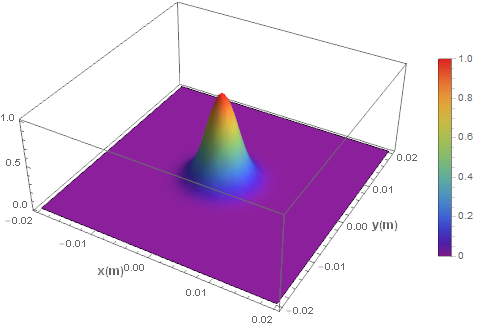
\includegraphics[width=0.45\linewidth]{gaussianbeam.png}
%\includegraphics[width=0.3\linewidth]{gaussianhuidu.png}
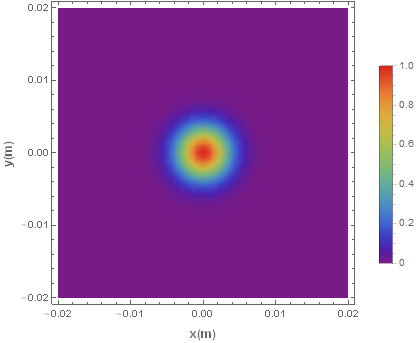
\includegraphics[width=0.45\linewidth]{gaussianbeamz=0.png}
\caption{束腰半径0.5mm的基模高斯光束}
\label{fig:gaussianbeam}
\end{figure}

对公式\eqref{eq:guangqiang}进行积分,同时将直角坐标系变换为极坐标系:$x=\omega(z)/\sqrt{2}\cdot\rho\sin\theta,y=\omega(z)/\sqrt{2}\cdot\rho\cos\theta$,能够得到z平面的光强:
\begin{equation}
\int_{-\infty}^{\infty}\int_{-\infty}^{\infty}I(x,y,z)\text{d}x\text{d}y=2A_0^2\int_0^{2\pi}\text{d}\theta\int_0^\infty\exp(-\rho^2)\rho\text{d}\rho=2\pi A_0^2
\end{equation}
式中,$A_0$为振幅,因此如果知道激光发射功率$P$,通过该式就能计算出高斯光束初平面的振幅,$A_0=\sqrt{P/2\pi}$。

事实上,在激光穿过流场时,会有能量的交换,激光对气体进行局部的加热从而损失一定的能量,如果用能量损耗系数$\beta$表示激光每传输一个单位的距离时相对损耗的功率,那么通过损耗系数就能够知道气体的升温率:
\begin{equation}
O(x,y,z)=\beta\cdot I(x,y,z)
\end{equation}
式中,$I(x,y,z)$表示空间上$(x,y,z)$点处的光强。

在通常情况下,谐振腔发出激光的振幅在横截面上的分布大多数呈现高斯函数的分布形式,而基模高斯光束在其中最具典型性,因此基模高斯光束的传输特性研究对于了解光学窗口处激光信号的接收发射具有重要意义。
\subsection{光波衍射的数值计算}
当光波经过小孔后,它的传输并不会按照线性光学理论所描述的会继续沿直线传播,而是会发生衍射现象,形成中心明亮的明暗相间的衍射圆环。一般衍射计量是利用夫琅禾费衍射作为依据的,夫琅禾费衍射又可以称作远场衍射,当平行光射入小孔时,在不同的传输距离上会出现不同的衍射光斑,光斑中心最亮,以第一圈暗环为分界线。中央的光斑强度占总强度的84\%左右,可以把这个中央亮斑称作爱里斑。当传输距离足够远时,光斑趋于稳定,随着距离的增加仅仅改变光斑半径,而衍射图样不发生变化,把这种衍射称为夫琅禾费衍射或远场衍射。

在第四章中经过流场作用后的夫琅禾费衍射可以由公式\eqref{eq:fraunhofer}表示,如果假设圆形小孔的直径为D,小孔的光学传递函数$OTF_D(x,y)$可以通过公式\eqref{eq:xiaokongguangchuandi}表示,点扩散函数可以表示为公式\eqref{eq:xiaokongdiankuosan}。
\begin{align}
OTF_D(x,y)&=\frac{2}{\pi}\Bigg[cos^{-1}\Big(\frac{\sqrt{x^2+y^2}}{D}\Big)-\frac{\sqrt{x^2+y^2}}{D}\sqrt{1-\Big(\frac{\sqrt{x^2+y^2}}{D}\Big)^2}\Bigg]
\label{eq:xiaokongguangchuandi}\\
PSF_D(x,y)&=\Bigg[2\cdot\frac{J_1\big[kD\sqrt{x^2+y^2}/(2L)\big]}{kD\sqrt{x^2+y^2}/(2L)}\Bigg]^2
\label{eq:xiaokongdiankuosan}
\end{align}
式中,由于小孔孔径外光学传递函数为零,因此需满足$\sqrt{x^2+y^2}\leq D/2$的条件。

通过公式\eqref{eq:xiaokongguangchuandi}、\eqref{eq:xiaokongdiankuosan}可以得到平面光波经过小孔衍射后的衍射光斑,如图\ref{fig:xiaokong}。事实上由于夫琅禾费衍射需要成立条件苛刻,需要在很远才能观测到衍射图案,实验条件难以达到,因此可以在小孔后面紧贴着放置一块焦距为d的透镜,将光波汇集到焦平面上,这样保证成像图案不变,仅改变了大小比例,由于一般仅需要观测夫琅禾费衍射的光斑分布,因此这种方法非常有效。
\begin{figure}[bhtp]
\centering
\subcaptionbox{直径为0.1cm的圆孔光学传递函数}{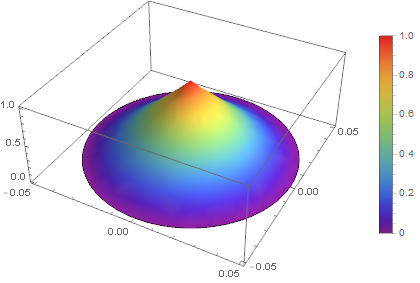
\includegraphics[width=0.45\linewidth]{xiaokongguangchuandi.png}}
\subcaptionbox{传输距离4km的夫琅禾费衍射}{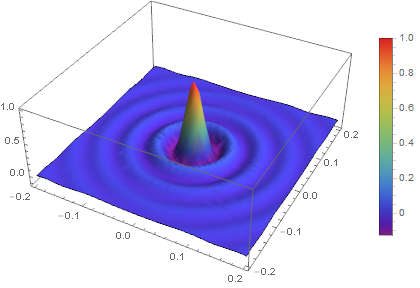
\includegraphics[width=0.45\linewidth]{fraunhofer.png}}
\caption{衍射孔光传递函数及夫琅禾费衍射}
\label{fig:xiaokong}
\end{figure}

由于实际流场结构的复杂性,通过上述衍射积分方法求解光学传递函数从而计算光场分布难以实现,通常情况下需要采用数值计算,为了在保证计算精度的同时简化计算量,可以采用稳相法来进行优化的数值计算,即采用渐进公式,利用代数运算替代复杂的积分公式。
\section{凸台光学窗口周围流场引起的光束畸变分析}
光束在湍流流场传播过程中的相位畸变主要是由于折射率脉动导致的,而折射率的脉动又由流场密度脉动引起,因此可以通过流场的密度脉动来求解相位畸变。通过$G-D$系数可以将密度与折射率联系起来,因此知道了流场密度,同时通过光线追迹法知道了光传输路径,就可以计算出光束的相位畸变。
\subsection{基于CFD网格的波面畸变计算}
由于在划分流场计算网格时,对边界层进行了加密处理,如图\ref{fig:tutaijiemianwangge}所示,因此从光学窗口到远离壁面之间的计算网格并非同样大小,越靠近光学窗口处网格越密,网格边长越小,本文以光学窗口中心为三维直角坐标系原点,形成$x-y$平面平行于窗口,$z$轴垂直于窗口平面的坐标系。

假设第$i$层网格上表面距离原点$l_i$,第$i+1$层网格上表面距离原点$l_{i+1}$,光线入射到第$i+1$层的入射角为$\theta_i$,根据直角三角形勾股定理以及直角余弦定理,可以近似地计算出光线在第$i$层网格中的实际传输距离$\Delta l_i$为$(|l_{i+1}-l_i|/\cos\theta_i)$
,每个网格中的折射率可以看作是前后表面折射率的算数平均即$(n_{i+1}+n_i)/2$,折射率差$\Delta n_i$可以定为$(n_{i+1}+n_i)/2-\bar{n}$,那么可以知道第$i$个网格中的光程差OPD应该为$\Delta l_i\cdot\Delta n_i$,对光束传播方向上的每一个网格中的光程差累加后就可以得到该条光线经过流场后的总的光程差:
\begin{equation}
\Delta L=\sum\limits_{i=1}^{\rm N}\frac{|l_{i+1}-l_i|}{\cos\theta_i}\cdot(\frac{n_{i+1}+n_i}{2}-\bar{n})
\label{eq:wanggegaungchengcha}
\end{equation}
式中,N为沿光传输方向的网格数量。

在计算光程差时,本文将网格沿光束传播方向分层,假定在同一层间传输方向不变,即如果光束在经过同一层不同网格时,仍保持传输方向,那么如果已知入射到第$i+1$层的入射角$\theta_i$,通过正弦定律可以得到第$i+2$层的入射角$\theta_{i+1}$,两者有如下关系:
\begin{equation}
(n_{i+1}+n_i)\cdot\sin\theta_i=(n_{i+2}+n_{i+1})\cdot\sin\theta_{i+1}
\label{eq:zhengxianjiao}
\end{equation}

通过式\eqref{eq:zhengxianjiao},给出初始入射角$\theta_0$就能经过计算得到光线入射到每一个网格面的入射角,将其反带入公式\eqref{eq:wanggegaungchengcha},进行离散的累加计算后,就能计算出每一条光线经过整个计算区域的光程差。
采用上述方法,对每一条光线进行追踪计算,得到了光学孔径上每一个入射到格点的光线光程差,通过对这些离散的光程差进行差值后,就能近似地得到时间平均的流场对光束在传播方向上的波面畸变情况。

通过第四章的理论分析,能够明确知道相位实际上是光程与波数的乘积,那么相位差就是光程差与波数的乘积,因此在给定波长的情况下,光波的光程差直接决定了光波相位畸变$\Delta \phi$的大小,如果入射光波波长为$\lambda$对应的光程差为$\Delta L$,那么光波的相位畸变可以写为如下表达式:
\begin{equation}
\Delta\phi=k\cdot\Delta L=\frac{2\pi}{\lambda}\cdot\Delta L
\label{eq:xiangweijibian}
\end{equation}

在基于CFD网格划分对光程差进行计算时,可以看出网格的划分情况对于计算至关重要,本文对机载光学凸台周围的网格按照流场流向划分,与Fluent的模拟结果较为契合,大大简化了基于直角三维坐标系的计算过程,对坐标系的建立能能够直接与网格走向一致。

以一倍音速以及两倍音速运行下的机载凸台光学设备周围流场为例,由于光学窗口大约位于凸台底部上方10cm左右,因此本文在凸台上方10cm处的近壁面取一个包含剪切层的流场,流场尺寸为长0.9m宽0.4m,高0.15m的长方体区域,查看不同速度下的波面畸变情况,图\ref{fig:zfangxiangguangchengcha}显示了不同速度下机载凸台光学窗口周围流场分布以及波面畸变情况,令x方向为飞行器前进方向。

\begin{figure}[bhtp]
\centering
\subcaptionbox{1Ma速度下流场底面及切面\label{fig:1matutaiqiemian}}{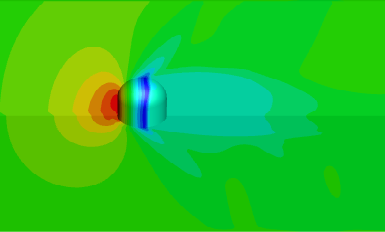
\includegraphics[width=0.48\linewidth]{1matutaicemian.PNG}}
\subcaptionbox{1Ma速度下光学窗口周围光程差\label{fig:tutaizhouweiguangchengcha1z}}{
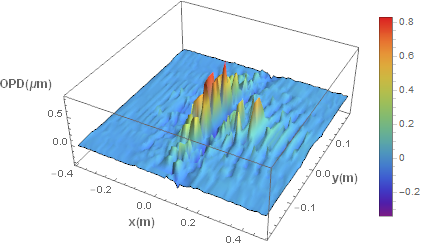
\includegraphics[width=0.48\linewidth]{tutaizhouweiguangchengcha1maz.png}}\\
\subcaptionbox{2Ma速度下流场底面及切面\label{fig:2matutaiqiemian}}{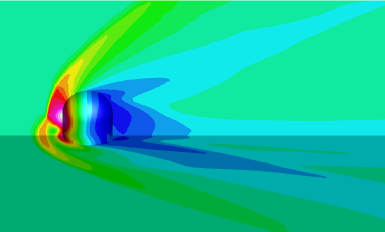
\includegraphics[width=0.48\linewidth]{2matutaicemian.PNG}}
\subcaptionbox{2Ma速度下光学窗口周围光程差\label{fig:tutaizhouweiguangchengcha2z}}{
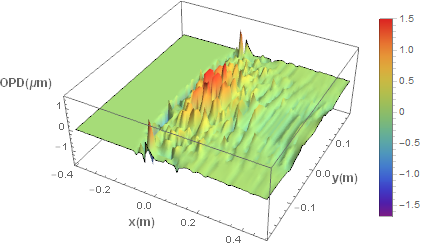
\includegraphics[width=0.48\linewidth]{tutaizhouweiguangchengcha2maz.png}}
\caption{不同速度下光束沿z方向传播的波面畸变}
\label{fig:zfangxiangguangchengcha}
\end{figure}

图\ref{fig:1matutaiqiemian}、\ref{fig:2matutaiqiemian}为通过计算流体力学软件模拟的两种不同速度下机载凸台底面以及中轴切面的流场密度分布情况,图\ref{fig:tutaizhouweiguangchengcha1z}、\ref{fig:tutaizhouweiguangchengcha2z}分别在一倍以及两倍音速下,光束沿z方向入射时,经过15cm厚的非均匀流场后在光学窗口处的波面畸变情况。可以发现当速度为1Ma时,沿z方向的光束光程差在$-0.3\mu\text{m}\sim0.8\mu\text{m}$之间波动,并且在凸台前方、周围近壁面及光学窗口后方的波面畸变较严重,而在2Ma运行速度下,光程差分布于$-1.6\mu\text{m}\sim1.5\mu\text{m}$之间,并且在凸台前方由于流场的压缩,光波仅在靠近壁面处产生畸变,随着速度的提升,波前畸变也会更加严重。

从图\ref{fig:tutaizhouweiguangchengcha1z}、\ref{fig:tutaizhouweiguangchengcha2z}能够发现在2Ma速度下光学窗口前方约12cm外的流场已经是均匀分布,这时光束在均匀流场中传输并不产生光程差,而1Ma下在更远处流场才呈现均匀性,因此在计算不同运行速度下飞行器的气动光学效应时,对于剪切层及湍流外边界的确定能够以此为参考。

由于图\ref{fig:zfangxiangguangchengcha}中计算了光束沿垂直于光学窗口方向入射进流场,经过15cm厚度的流场后的光程差,而在大多数情况下,探测光线一般比较靠近飞行器前进方向,即与光学窗口轴向成较大的角度入射进光学探测窗口,为此,可以对比不同角度的入射光束的波面畸变情况,如图\ref{fig:xgangxiangguangchengcha}所示。

\begin{figure}[bhtp]
\centering
\subcaptionbox{1Ma速度下光学窗口周围光程差\label{fig:tutaizhouweiguangchengcha1x}}{
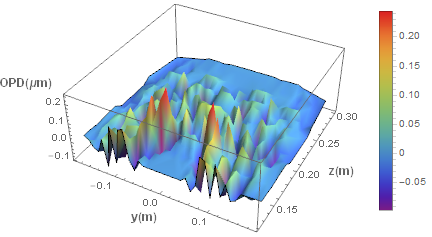
\includegraphics[width=0.48\linewidth]{tutaizhouweiguangchengcha1max.png}}
\subcaptionbox{2Ma速度下光学窗口周围光程差\label{fig:tutaizhouweiguangchengcha2x}}{
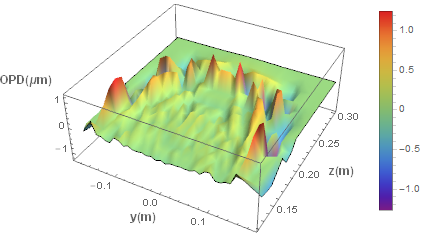
\includegraphics[width=0.48\linewidth]{tutaizhouweiguangchengcha2max.png}}
\caption{不同速度下沿前进方向产生的波面畸变}
\label{fig:xgangxiangguangchengcha}
\end{figure}

图\ref{fig:xgangxiangguangchengcha}分别显示了不同速度下,沿着飞行器前进方向传播的光束产生的光程差,由于沿前进方向的流场结构不同于垂直于前进方向的流场结构,根据图\ref{fig:midudaozheshelv}所示,在光学窗口前方约6cm处流场就已经可以看作为均匀远场状态,因此对于沿前进方向入射的光束,层流区域的选择需要进行相应的改变。

本文取机载凸台前方0至7cm厚度的长方体区域作为研究区域,对不同速度下的波面畸变进行计算,如图\ref{fig:tutaizhouweiguangchengcha1x}、\ref{fig:tutaizhouweiguangchengcha2x}所示,可以看出1Ma速度下光程差于-0.1$\mu{\rm m}\sim$0.25$\mu$m之间,2Ma下光程差位于-0.5到1.9$\mu$m之间,凸台周围的波面发生严重畸变。

对比图\ref{fig:zfangxiangguangchengcha}和图\ref{fig:xgangxiangguangchengcha}可以发现沿前进方向的光程差明显小于z方向的光程差,这和流场厚度有一定关系,同时也与流场在不同方向的结构不同有关,因此入射角度影响了高速飞行器周围流场的分析。

由公式\eqref{eq:xiangweijibian}可以看出相位差与光程差成正比关系,与波长成反比关系,由此推测,如果给定流场结构以及光波进入流场的方向,那么入射光波波长越大,流场引起的相位差越小,从而导致波前畸变越小,因此可以认为对于给定的流场,入射光波波长越大越好,但是由于激光能量与光波波长存在相反的关系,波长越长的光波能量越小,强度越弱,因此如何选定探测波长也成为比较关键的问题。
\subsection{基于斯特列尔比及光传递函数的光束质量分析}
斯特列尔比作为一个重要的气动光学评价指标,可以通过波面误差来计算,如公式\eqref{eq:strehljunfangcha}所示,而该公式中相位均方差的计算则相应地能够通过密度均方差来求解,从而计算出流场的斯特列尔比。

本节参考上节计算光束波面畸变的处理方法,主要基于网格格点数据离散的方式对斯特列尔比进行分层的叠加求解,合理地假设光学孔径尺寸远大于流场密度脉动尺寸,在此假设基础上求解出斯特列尔比及光学传递函数,分析光束经过流场前后的能量损失情况,并且给出流场对光学成像的影响分析。

\begin{figure}[bhtp]
\centering
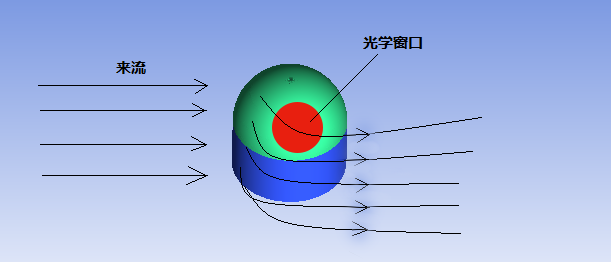
\includegraphics[width=0.9\linewidth]{tutaichuangkou.PNG}
\caption{机载凸台光学窗口示意图}
\label{fig:guangxuechaungkou}
\end{figure}

本文在对凸台光学窗口周围流场的气动光学效应进行计算时,根据凸台光学窗口距离底部的高度情况,选取了离凸台底部10cm高的光学探测窗口所处的流场区域,凸台光学窗口如图\ref{fig:guangxuechaungkou}所示。如果将流场厚度记为H,可以将非均匀流场划分为N个薄层,每层厚度为$h=$H/N,并且$h$大于湍流的涡旋尺度$l$,湍流的涡旋尺度根据在流场模拟中选用的模型的不同,也相应的有不同的经验估计方法,一般可以用$k-\varepsilon$和$k-\omega$模型的经验公式\eqref{eq:tuanliuchidu}。
\begin{equation}
\left\{
\begin{aligned}
&l=\frac{k^{3/2}}{\varepsilon}\cdot\frac{uL}{Re}~~~~~~~~&(k-\varepsilon\text{模型})\\
&l=\frac{k^{1/2}}{0.09\omega}\cdot\frac{uL}{Re}~~~~~~~~&(k-\omega\text{模型})
\end{aligned}
\right.
\label{eq:tuanliuchidu}
\end{equation}
式中,$u$为远场来流速度,$L$为飞行器结构长度,$Re$为雷诺数。

在计算密度均方差$\sigma_\rho^2$时,假定$\rho(x,y,z)$只取决于传输距离$z$而与孔径坐标$(x,y)$无关,那么就可以认为密度脉动均方差与$z$相关,记为$\sigma_\rho^2(z)$,同时记湍流在z方向的脉动尺度为$l_z(z)$,可以将相位均方差表示为如下公式所示:
\begin{equation}
\sigma_\phi^2\approx2K_{GD}^2\int_0^{\rm H}\sigma_\rho^2(z)l_z(z)\text{d}z
\end{equation}

在基于CFD软件模拟后的流场基础上计算时,可以通过网格格点将相位均方差公式离散,对传输方向每个网格面上的密度脉动均方差累加就能得到最终整个光瞳区域的密度脉动均方差,从而得到相位均方差:
\begin{equation}
\sigma_\phi^2\approx2K_{GD}^2\sum\limits_{i=1}^{N}\big[h_i\cdot\sigma_{\rho i}^2\cdot l_{zi}\big]
\label{eq:lisanxiangweimaidong}
\end{equation}
式中,$h_i$为沿传播方向第$i$层网格宽度,$\sigma_{\rho i}^2$表示第$i$层网格面上的密度脉动均方差,$l_{zi}$为z方向第$i$个网格处的脉动尺度。

利用离散点的相位均方差公式,结合大孔径近似下的斯特列尔比,见公式\eqref{eq:strehljunfangcha},就能够计算得到孔径为D的光学光口处斯特列尔比,也就是光束穿过流场后的产生像差后的中心光强与没有像差时中心光强的比值,这个比值显示了像点的分辨能力,从而可以对流场的气动光学效应做出相应的评估。

由于光束入射角度的不同,光束在流场中的传输路径也是不同的,这就导致光斑的光强分布随着入射角度的变化而变化,因此可以考虑几种不同的入射角,分别分析经过流场后的斯特列尔比。

本文以2Ma运行速度下的机载凸台为例,为了便于结合网格进行计算,在凸台光学窗口处截取了8$\times$8cm的方形光学孔径,根据第三章中的流场数值模拟结果,确定光学窗口处流场厚度为10cm,计算了垂直入射到光学孔径平面的光束产生的光程差,其等值图如图\ref{fig:chuangkoujibian}所示。

\begin{figure}[bhtp]
\begin{minipage}[b]{0.45\linewidth}
\centering
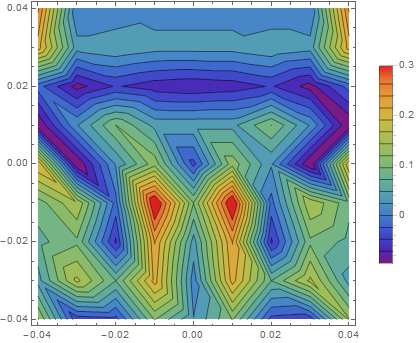
\includegraphics[width=\linewidth]{xiangweijibian.png}
\caption{光学窗口波面畸变($\mu$m)}
\label{fig:chuangkoujibian}
\end{minipage}
\begin{minipage}[b]{0.5\linewidth}
\centering
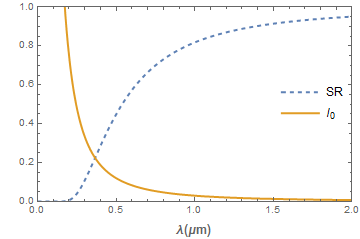
\includegraphics[width=\linewidth]{lixiangbizhi.png}
\caption{理想光强与斯特列尔比}
\label{fig:lixiangsite}
\end{minipage}
\end{figure}

采用公式\eqref{eq:lisanxiangweimaidong}的方法计算得到了相应的斯特列尔比约为25.37\%。为了进行对比,本文同时计算了光束在10$\textdegree$和20$\textdegree$两种不同角度下入射进光学窗口时的斯特列尔比分别为23.26\%和21.35\%,对比可以看出入射角度的变化一定程度上影响了光学成像质量,入射角越小,光束中心越亮,成像质量越好。


由于通过斯特列尔比表达式以及上述计算能够分析出在给定流场及入射角度情况下,斯特列尔比SR与光束波长平方的倒数成负指数关系($SR\propto\exp(-1/\lambda^2)$),而光强$I_0$与光束波长平方的倒数成正比关系($I_0\propto\dfrac{1}{\lambda^2}$),如图\ref{fig:lixiangsite}所示,图中的曲线仅表示光强与斯特列尔比的走势,实线为斯特列尔比随波长变化情况,虚线表示光强随波长变化情况,从对比图可以看出合适的探测波长选择也成为影响成像质量的重要因素,并且大量实验证明小于波长2$\mu$m的光波受到的气动光学效应影响比较严重。

通过第四章的理论分析,流场对光传输的作用能够分为平均流场部分和湍流随机脉动部分的综合作用,如果令平均流场以及脉动流场部分的光学传递函数分别为$f_{OTF1}(x,y),f_{OTF2}(x,y)$,那么两者对应相乘即可表示整个流场的光传递函数$f_{OTF}(x,y)=f_{OTF1}(x,y)\times f_{OTF2}(x,y)$,根据公式\eqref{eq:guangtonghanshu}定义光瞳函数$f(x,y)$为与光程差相关的函数,并且仅在光瞳孔径范围内存在,超出孔径范围则为零,那么通过光瞳函数自相关积与光传递函数存在等量关系,如公式\eqref{eq:pingjunguangchuandi}。
\begin{equation}
\left\{\begin{aligned}
&f_{OTF1}(x,y)=\frac{1}{S}\cdot f(x,y)*f(x,y)~~~~~~~~(x,y)\in {\rm A}\\
&f(x,y)=\exp(-i\Delta\phi)=\exp(-ik\Delta L)
\end{aligned}
\right.\label{eq:pingjunguangchuandi}
\end{equation}
式中,$S$是光学孔径的面积,A表示光学孔径区域,$\Delta L$表示光程差,$*$表示卷积。

而对于湍流随机脉动部分来说,光学传递函数主要与折射率的脉动起伏有一定的函数关系,
\begin{equation}
f_{OTF2}(x,y)=\exp\Big[-2k^2\int_0^H\overline{n'^2}(x,y,z)\cdot\big[l_{xyz}-\int_0^\infty C(x',y',z'){\rm d}z'\big]{\rm d}z\Big]
\label{eq:maidongguangchuandi}
\end{equation}
式中,本文选取指数模型的湍流相关系数$C(x',y',z')$,见公式\eqref{eq:zhishuxiangguanxishu},$\overline{n'^2}$为流场折射率脉动,可以通过流场密度分布求解,横向积分尺度$l_{xyz}$可以选择相应经验公式求解,本文采用公式\eqref{eq:tuanliuchidu}中的$k-\omega$模型的经验公式计算,经验公式中的流场基本参数主要由第三章中的凸台周围流场模拟部分给出。

因此,如果能够知道初始光束的表达式,通过公式\eqref{eq:pingjunguangchuandi}和公式\eqref{eq:maidongguangchuandi}得到整个流场的光学传递函数,就能给出经过流场后的光斑光强分布情况,如公式\eqref{eq:guangqiangfenbu}。
\begin{equation}
I(x',y')=\frac{1}{\lambda^2H^2}\iint\limits_{\rm A}I_0(x,y)f_{OTF}(x,y)\cdot\exp\big[\frac{2\pi}{\lambda H}(xx'+yy')\big]{\rm d}x{\rm d}y
\label{eq:gaungqiangfenbu}
\end{equation}
式中,由于传输距离较短,近似地将流场厚度$H$等价于光束实际路程,在基于网格计算时,需要将连续的积分公式转换为网格点的数值累加计算,如下所示:
\begin{equation}
I(x',y')=\sum\limits_{z=1}^{N}\frac{1}{\lambda^2h_z^2}\sum\limits_{i=1}^{N_x}\sum\limits_{j=1}^{N_y}I_0(x_i,y_j)f_{OTF}(x_i,y_j)\cdot\exp\big[\frac{2\pi}{\lambda h_z}(x_ix'+y_iy')\big]\cdot\Delta x\Delta y
\label{eq:gaungqiangfenbu1}
\end{equation}
式中,将流场分为N层,每层厚度为$h_z$,本文对近壁面处网格进行了加密,因此越靠近壁面,网格厚度$h_z$越小,每层网格在光学孔径上划分$N_x\times N_y$个小网格,网格边长分别为$\Delta x,\Delta y$。

本文将进入流场前的激光光束定义为束腰半径是1cm的基模高斯光束,截面光强分布满足高斯分布,如式\eqref{eq:guangqiang}所示,可以得到初平面的光强分布如图\ref{fig:chushigaosi}所示,采用式\eqref{eq:pingjunguangchuandi}、式\eqref{eq:maidongguangchuandi}以及式\eqref{eq:guangqiangfenbu}联立,代入公式\eqref{eq:gaungqiangfenbu1}后,通过基于网格格点的离散计算,同样对每段传输过程进行分层处理,并对结果进行归一化。计算区域为上述选定的厚度为10cm的流场区域,光束沿与光学窗口平面30\textdegree 角入射,光束偏移量通过上节光程差计算方法得到,通过平均及脉动流场叠加得到的光学传递函数$f_{OTF}$计算出了像平面的光强分布如图\ref{fig:jibiangaosi}所示。
\begin{figure}[bhtp]
\centering
\subcaptionbox{初平面高斯光束\label{fig:chushigaosi}}{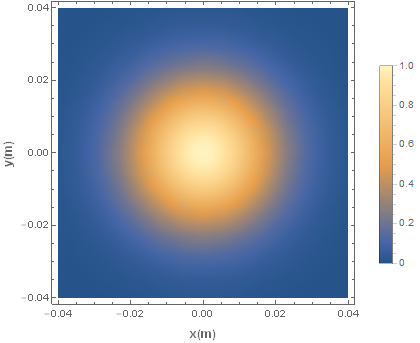
\includegraphics[width=0.45\linewidth]{yuanguangshu.png}}
\subcaptionbox{产生畸变后的高斯光束\label{fig:jibiangaosi}}{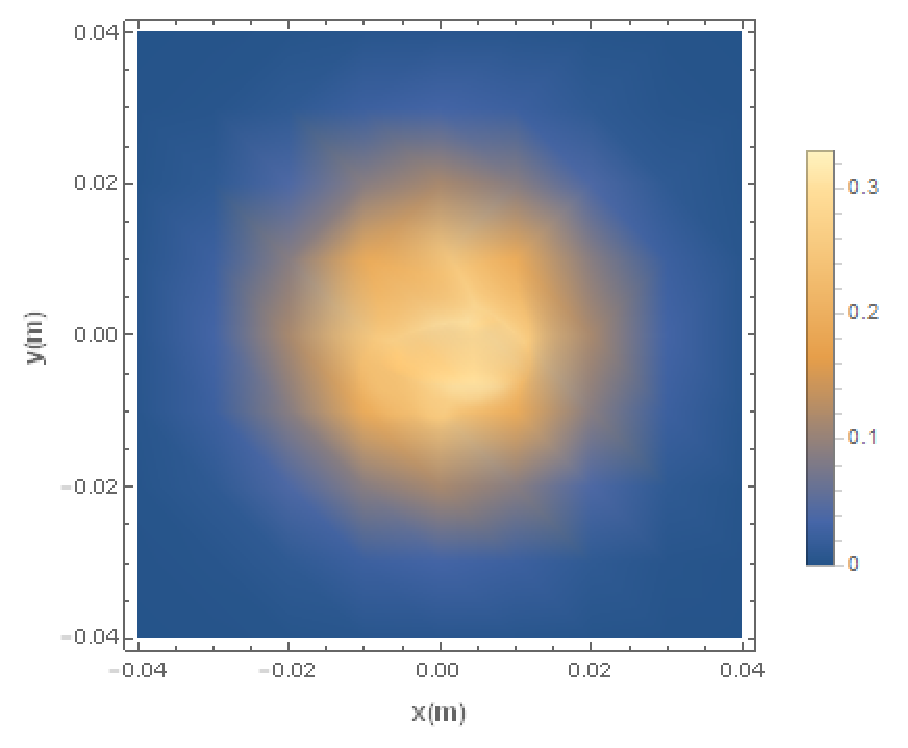
\includegraphics[width=0.45\linewidth]{pianyiguangshu.eps}}
\caption{高斯光束经过流场后的光场分布情况}
\end{figure}

通过对比光束经过凸台光学窗口周围流场前后的光斑情况,发现光斑中心亮度明显减弱,并且光场分布不再满足高斯分布,光强的分布受到整个流场在光学孔径上的光学传递函数影响,呈现不规则分布,光斑整体略有偏移,中心沿xy方向上的偏移距离为(0.022cm,-0.013cm),由此发现混合流场对于短距离成像的偏移作用很小,但是对于远距离传输情况而言,目标的成像及定位会因此产生较大的偏移。至此,通过斯特列尔比以及光学传递函数,较为明确地评价了光束经过流场的传输效应,为将来的光学校正提供了基础。
\section{本章小结}
本章基于Mathematica数据处理,通过Gladstone-Dale定律,完成了从流场参数到光学参数的转换,分析了2Ma运行速度下机载光学设备周围流场的折射率分布情况。对在实际应用中广泛使用的高斯光束的传播特性进行了研究并对其模拟成像,另外对圆形光学孔径的点扩散函数及光学传递函数进行了公式推导及计算,同时计算了远场夫琅禾费衍射的衍射图。最后对机载凸台周围的流场进一步分析,基于CFD计算网格的划分,讨论了流场对光波传输后的波面畸变的影响以及斯特列尔比的评价计算方法,对流场的气动光学效应进行了评估,计算了流场的光学传递函数,给出了高斯光束穿过流场后的光强分布情况。%--第四章--
%\chapter{结论及展望}
\section{本文总结}
本文主要通过理论分析以及数值模拟的研究方法对高速飞行器周围流场的物理特性以及流场引起的气动光学效应进行了研究,得到结论如下:

(1)基于流体力学理论,在假设高速湍流流场满足N-S方程组以及完全气体状态理论的基础上,对大涡模拟及雷诺平均法进行了推演,并通过对雷诺应力建立计算模型完成流场的分析。基于$k-\varepsilon$模型及$k-\omega$模型的混合算法推导出了剪切应力传输(SST)模型,另外讨论了在高超声速情况下的流场运动特征,指出在高超声速情况下流体性质发生变化且不再满足上述假设,应考虑真实气体效应和气动加热等问题。

(2)设定了流体运动方程组数值计算前的定解条件,利用隐式迭代法对控制方程进行了离散,通过ICEM建立了三维导弹、机载光学凸台的模型,对近壁面流场的网格进行了加密优化处理。通过Fluent对不同运行速度下的流场进行了数值模拟,得到流场各项物理参数,并发现在超音速情况下剪切层随速度增加而越来越靠近飞行器壁面,同时基于完整的分析过程建立了流场数值模拟以及分析的具体流程。

(3)基于光的波动理论及线性光学理论分析了光束在非均匀流场中的传输特性,介绍了在时均流场中常用的光线追迹法以及推导了在湍流流场中的基于折射率脉动的统计光学研究方法。提出在气动光学效应的计算中可以在时间平均流场中引入网格模型以及在湍流部分引入亚格子尺度模型,讨论了混合后的非均匀流场的光学传递函数计算方法并且研究了偏折角、斯特列尔比等气动光学计算及评价方法。

(4)基于CFD的数值模拟结果,完成了密度到折射率的直接转换,讨论了高斯光束的传播特性及夫琅禾费衍射特征,利用Mathematica计算了在不同速度、不同入射角下光学窗口周围的光束波面畸变,发现沿前进方向射入光学窗口的光束波面畸变远远小于垂直于前进方向产生的波面畸变,并计算出不同入射角下运行速度为2Ma时光学孔径范围内的斯特列尔比在0.21至0.26之间浮动。采用光学传递函数计算得到了高斯光束经过混合流场前后的光斑变化,发现经过2Ma下凸台光学窗口处10cm厚的流场作用后,光束在像面上的光强不再成高斯分布,并且光束中心偏移量为(0.022cm,-0.013cm)。

本论文完成了不同速度下飞行器周围流场的数值模拟,将得到的流场结果转化为光学参数,基于光学传输的理论模型计算了光束经过高速湍流流场后的畸变情况,并对结果进行了分析,为进一步实际应用中的光学校正以及气动光学效应的削弱提供了有力基础。
\section{对未来工作的展望}

本文有待进一步的研究工作:

(1)通过风洞试验对数值模拟结果进行验证,同时增加对高超声速情况下的流场机理研究,考虑真实气体效应、气动加热等问题对光传输的影响。

(2)对气动光学的评价方法上进行改进,并且结合远场成像,完成对光信号的实际接收以及目标成像、跟踪。%--第四章--
}
%------正文结束------------
%-----致谢、参考文献、附录---开始-----
\clearpage
\phantomsection
\addcontentsline{toc}{chapter}{致~~~~~~~~谢}%--致谢加入目录---
\chapter*{\markboth{致谢}{致谢}致~谢}
本论文是在我的导师赵琦教授的耐心指导以下完成的,从课题的选取到论文的撰写,赵老师付出了大量的心血,从导师身上我不仅学到了严谨、科学的研究方法,更收获到了为人处世的道理,导师在我迷茫的时候给我指引了前进的道路,给予我很大的鼓励,在此向赵老师表示最诚挚的谢意。

同时还要感谢课题组的陈延如教授、 辛煜老师和周木春老师在我的学习生涯中给予的无私帮助,让我的论文能够顺利完成。感谢张淇博博士以及教研室同学在学习工作中的陪伴,让我从他们身上获取了强大的精神力量,感谢两位室友钱国鹏、张伟良在我生活中的陪伴,让我在日常生活中能快乐地度过。

感谢Donald E. Knuth先生发明的\TeX 排版系统,Stephen Wolfram先生发明的Mathematica数学计算软件,以及ANSYS公司研制的有限元分析软件,这些优秀的科研工具为我的论文撰写和科学研究提供了巨大的帮助。

感谢我的父亲、母亲、哥哥、嫂子还有可爱的侄女,他们是世界上最爱我以及我最爱的人,给了我一个温暖快乐、积极向上的家庭,这是我在外漂泊、求学过程中内心深处最安稳的栖息地。

最后感谢我自己,能够健康、快乐地成长为世间独一无二、想法奇特、喜欢思考、感性与理性并存的我。




%--致谢-------	
\clearpage
\phantomsection
\addtolength{\bibsep}{-0.5em}
\addcontentsline{toc}{chapter}{参考文献}
%--参考文献加入目录--
\setlength{\baselineskip}{18pt}
\bibliography{body/reference/nantong}%--参考文献---
\clearpage
\phantomsection
\addcontentsline{toc}{chapter}{附~~~~~~~~录}%--附录加入目录---
\chapter*{\markboth{附录}{附录}附录}
\setlength{\baselineskip}{20pt}
\noindent {\bfseries\large 在攻读硕士学位期间,本人取得学术成果如下:}

\begin{enumerate}
\renewcommand\labelenumi{[\theenumi]} 
\item {\bfseries ZHU ZhengTian}, ZHANG MingMing, ZHAO Qi, et al. Propagation properties of off-axis elliptical vortex beams[EB/OL]. Beijing:
Sciencepaper Online[2014-09-10]. http://
www.paper.edu.cn/
release paper/content/201409-123.
\item 冯嘉文,{\bfseries 朱正天},赵琦,陈元恺,刘一斯.离轴参量及传输距离对离轴涡旋光束传输特性的影响[J].中国科技论文在线精品论文,2015,8(15):1581-1586

(国内统一刊号:CN11-9150/N5~,~国际标准刊号:ISSN1674-2850)
\item {\bfseries ZhengTian Zhu},Qi Zhao,QiBo Zhang,XinYu Peng,Dong Ye. Analysis of aero-optical effect around the turbulent flow field of the high-speed aircraft[J].Optical and Quantum Electronics.(审核中)
\end{enumerate}

\noindent {\bfseries\large 攻读硕士学位期间参与的科研基金项目:}
\begin{enumerate}
\item 高等学校博士学科点专项科研基金(20123219110021)
\item 上海航天科技创新基金(SAST201350)
\end{enumerate}
%--附录----
%------致谢、参考文献、附录---结束------
%-----------------文章完毕--------------
\end{document}